\documentclass[a4paper, 12pt]{report}

\usepackage{graphicx}
\usepackage{ucs}
\usepackage[utf8x]{inputenc}
\usepackage[T1]{fontenc}
\usepackage[ngerman]{babel}
\usepackage[a4paper, left=2.5cm, right=2cm, top=2cm, bottom=2cm]{geometry}
\usepackage{amsmath}
\usepackage{multicol}
\usepackage{tikz}
\usetikzlibrary{arrows,decorations.pathmorphing,backgrounds,fit,positioning,
shapes.symbols,chains,shapes.geometric,shapes.arrows,calc}

\title{Prüfungsvorbereitung für die IHK-Abschlussprüfung Teil I}
\author{L.M.}

\begin{document}
\maketitle

\tableofcontents

\newpage
\chapter{Entwicklung vernetzter Prozesse}
\begin{multicols}{2}
\section{Elektrotechnik}
\subsection{Grundgrößen der Elektrotechnik}

\paragraph{Die Elektrische Spannung:}

\begin{center}
	\begin{tabular}{ ll }
		Formelzeichen & U            \\
		Einheit       & Volt (V)     \\
		Beispiel      & $U = 230V$ \\
	\end{tabular}
\end{center}

\paragraph{Die Elektrische Stromstärke:}

\begin{center}
	\begin{tabular}{ ll }
		Formelzeichen & I            \\
		Einheit       & Ambere (A)   \\
		Beispiel      & $I = 2A$    \\
	\end{tabular}
\end{center}

\paragraph{Der Elektrische Widerstand:}

\begin{center}
    \begin{tabular}{ ll }
		Formelzeichen & R            \\
		Einheit       & Ohm ($\Omega$)   \\
		Beispiel      & $R = 10\Omega$    \\
	\end{tabular}
\end{center}

\paragraph{Das Ohmsche Gesetz:}

\begin{center}
    \begin{equation}
	U = R \cdot I
    \end{equation}
    \begin{equation}
	P = U \cdot I
    \end{equation}
\end{center}

\subsection{Mathematische Zusammenhänge der Reihenschaltung}

In einer \emph{Reihenschaltung} fließt der Strom durch einen Widerstand nach
dem anderen. Daraus ergeben sich folgende Zusammenhänge:

\begin{center}
    \begin{equation}
	U_G = U_1 + U_2 + \dots + U_n
    \end{equation}
    \begin{equation}
	I_G = I_1 = I_2 = I_3 = \dots = I_n
    \end{equation}
    \begin{equation}
	R_G = R_1 + R_2 + \dots + R_n
    \end{equation}
\end{center}

Da alle Elektronen, die durch Widerstand No. 1 fließen, auch durch alle
folgenden Widerstände fließen müssen. An der \emph{Stromstärke} an sich ändert
sich nichts. Der Gesamtwiderstand und die Gesamtspannung ist aus selbigem Grund
die \emph{Summe aller Teilwiderstände bzw. -Spannungen}.

\subsection{Mathematische Zusammenhänge der Parallelschaltung}

In einer \emph{Parallelschaltung} werden Widerstände und/oder Kondensatoren
parallel in einem Schaltkreis angeordnet. Bei jeder Abzweigung \emph{teilt
sich der Strom auf}. Daraus ergeben sich folgende Zusammenhänge:

\begin{center}
    \begin{equation}
	I_G = I_1 + I_2 + \dots + I_n
    \end{equation}
    \begin{equation}
	U_G = U_1 = U_2 = \dots = U_n
    \end{equation}
    \begin{equation}
	\frac{1}{R_G} = \frac{1}{R_1} + \frac{1}{R_2} + \dots + \frac{1}{R_n}
    \end{equation}
\end{center}

In der Parallelschaltung bleibt also die \emph{Spannung konstant}, und die
Stromstärke lässt sich durch die Aufteilung der Gesamtstromstärke
\emph{aufaddieren}. Es gilt zu beachten, dass der Widerstand nicht \emph{größer},
sondern \emph{kleiner} wird, je mehr Widerstände parallel geschaltet werden.
Der Grund dafür wird klar, wenn man sich den Widerstand als Tür vorstellt - es
können \emph{mehr Menschen} hindurchgehen, je mehr \emph{Türen} es gibt.

Auch hier gilt das Ohmsche Gesetz. Für den Spezialfall von zwei parallel
geschalteten Widerständen kann die Formel für den Gesamtwiderstand umgestellt
werden. Es gilt damit:
\begin{center}
    \begin{equation}
	R_G = \frac{R_1 \cdot R_2}{R_1 + R_2}
    \end{equation}
\end{center}

\subsection{Elektrizitätszähler}

Elektrizitätszähler, bzw. Energiezähler oder Kilowattstundenzähler dienen zur
Messung der elektrischen Energie, die man im Haushalt oder in der Industrie
aus dem Stromnetz bezieht.

Die elektrische Arbeit wird direkt mit einem Elektrizitätszähler gemessen.
Die Anzeige erfolgt digital in der Einheit kWh.

Für jeden Zähler wird eine Zählerkonstante $C_Z$ angegeben, aus der man
entnehmen kann, wieviele Umdrehungen der Zählerscheibe (im falle eines
mechanischen Zählers) bzw. wieviele Impulse der LED (Im Falle eines
elektronischen Zählers) einer kWh entscpricht.

Für den mechanischen Zähler gilt:

\begin{center}
    \begin{equation}
	C_Z = \frac{Umdrehungen}{kWh}
    \end{equation}
\end{center}

Für den elektronischen Zähler gilt:
\begin{center}
    \begin{equation}
	C_Z = \frac{Impulse}{kWh}
    \end{equation}
\end{center}

Außerdem gilt folgendes über die elektrische Arbeit (Watt):
\begin{center}
    \begin{equation}
	W = \frac{n}{C_Z}
    \end{equation}
\end{center}

Wobei $n$ der Anzahl Umdrehungen bzw. Impulsen entspricht.

Zur Messung der elektrischen Leistung zählt man die Umdrehungen/Impulse pro
Minute und rechnet dann hoch auf die Stunde. Die Leistung errechnet sich dann
aus:

\begin{center}
    \begin{equation}
	P = \frac{W}{t} = \frac{n}{C_Z \cdot t}
    \end{equation}
\end{center}

Oder zur direkten Berechnung in kW:

\begin{center}
    \begin{equation}
	P = \frac{1}{\frac{1}{kWh} \cdot h} = kW
    \end{equation}
\end{center}

\section{Digitaltechnik}

\subsection{Grundverknüpfungen in der Digitaltechnik}

\subsubsection{UND/AND/Konjunktion}

Das \emph{UND} ist eine Grundverknüpfung, die nach dem Prinzip
\emph{"Wenn A und B, dann..."} funktioniert. Der Ausgang $Q$ ist dann immer 1,
wenn die Eingänge $A$ und $B$ gleich 1 sind. Das \emph{UND} wird auch als
\emph{Konjunktion} bezeichnet und wird im Englischen \emph{AND} genannt.

\begin{center}
    \begin{equation}
	Q = A \land B
    \end{equation}
    \begin{tabular}{ | c | c || c | }
    	\hline
    	A & B & Q \\ \hline
    	0 & 0 & 0 \\ \hline
    	0 & 1 & 0 \\ \hline
    	1 & 0 & 0 \\ \hline
    	1 & 1 & 1 \\
    	\hline
    \end{tabular}
\end{center}

\subsubsection{ODER/OR/Disjunktion}

Das \emph{ODER} ist eine Grundverknüpfung, die nach dem Prinzip
\emph{"Wenn eine der möglichen Bedingungen war sind, dann ist das Ergebnis
wahr"} arbeitet. Der Ausgang Q ist dann immer 1, wenn mindestens einer der
Eingänge $A$ und $B$ 1 sind. Das \emph{ODER} wird als Disjunktion bezeichnet
und wird im Englischen \emph{OR} genannt.

\begin{center}
    \begin{equation}
	Q = A \lor B
    \end{equation}
   \begin{tabular}{ | c | c || c | }
    	\hline
    	A & B & Q \\ \hline
    	0 & 0 & 0 \\ \hline
    	0 & 1 & 1 \\ \hline
    	1 & 0 & 1 \\ \hline
    	1 & 1 & 1 \\
    	\hline
    \end{tabular}
\end{center}

\subsubsection{NICHT/NOT/Negation}

Das \emph{NICHT} ist eine Grundverknüfung, die nach dem Prinzip \emph{"Wenn ein
Zustand oder eine Aussage wahr ist, dann ist das Ergebnis unwahr"} arbeitet.
Das \emph{NICHT} wird als Negation bezeichnet und wird im Englischen \emph{NOT}
genannt.

\begin{center}
    \begin{equation}
	Q = \neg A
    \end{equation}
	\begin{tabular}{ | c || c | }
		\hline
		A & Q \\ \hline
		0 & 1 \\ \hline
		1 & 0 \\
		\hline
	\end{tabular}
\end{center}

\subsubsection{NICHT-UND/NAND/NUND}

Das \emph{NICHT-UND} ist eine aus \emph{UND} und \emph{NICHT}
zusammengeschaltete Verknüpfung, welche das Ergebnis einer \emph{UND}
Verknüpfung negiert. Das \emph{NICHT-UND} wird auch als \emph{NUND}
bezeichnet und wird im Englischen \emph{NAND} genannt.

\begin{center}
    \begin{equation}
	Q = \neg(A \land B)
    \end{equation}
    \begin{equation}
	\neg Q = A \land B
    \end{equation}
   \begin{tabular}{ | c | c || c | }
    	\hline
    	A & B & Q \\ \hline
    	0 & 0 & 1 \\ \hline
    	0 & 1 & 1 \\ \hline
    	1 & 0 & 1 \\ \hline
    	1 & 1 & 0 \\
    	\hline
    \end{tabular}
\end{center}

\subsubsection{NICHT-ODER/NOR/NODER}

Das \emph{NICHT-ODER} ist eine aus \emph{ODER} und \emph{NICHT}
zusammengeschaltete Verknüpfung, welche das Ergebnis einer \emph{ODER}
Verknüpfung negiert. Das \emph{NICHT-ODER} wird auch als \emph{NODER}
bezeichnet und wird im Englischen \emph{NOR} genannt.

\begin{center}
	\begin{equation}
		Q = \neg(A \lor B)
	\end{equation}
	\begin{equation}
		\neg Q = A \lor B
	\end{equation}
   \begin{tabular}{ | c | c || c | }
    	\hline
    	A & B & Q \\ \hline
    	0 & 0 & 1 \\ \hline
    	0 & 1 & 0 \\ \hline
    	1 & 0 & 0 \\ \hline
    	1 & 1 & 0 \\
    	\hline
    \end{tabular}
\end{center}

\subsubsection{Exklusiv-ODER/XOR/Antivalenz}

Das \emph{Exklusiv-ODER} ist ein zusammengeschaltetes Element aus \emph{XNOR}
und \emph{NICHT}, welches das Ergebnis einer \emph{XNOR} Verknüpfung negiert.
Das \emph{Exklusiv-ODER} wird auch als Antivalenz bezeichnet und wird im
Englischen \emph{XOR} genannt.

\begin{center}
	\begin{equation}
		Q = (\neg A \land B) \lor (A \land \neg B)
	\end{equation}
   \begin{tabular}{ | c | c || c | }
    	\hline
    	A & B & Q \\ \hline
    	0 & 0 & 0 \\ \hline
    	0 & 1 & 1 \\ \hline
    	1 & 0 & 1 \\ \hline
    	1 & 1 & 0 \\
    	\hline
    \end{tabular}
\end{center}

\subsubsection{Exklusiv-NICHT-ODER/XNOR/Äquivalenz}

Das \emph{Exklusiv-NICHT-ODER} ist eine zusammengeschaltete Verknüpfung, dessen
Ausgang immer dann 1 ist, wenn alle Eingänge 2 sind. Das
\emph{Exklusiv-NICHT-ODER} wird auch als Äquivalenz bezeichnet und wird im
Englischen \emph{XNOR} genannt.

\begin{center}
	\begin{equation}
		Q = (A \land B) \lor (\neg A \land \neg B)
	\end{equation}
   \begin{tabular}{ | c | c || c | }
    	\hline
    	A & B & Q \\ \hline
    	0 & 0 & 1 \\ \hline
    	0 & 1 & 0 \\ \hline
    	1 & 0 & 0 \\ \hline
    	1 & 1 & 1 \\
    	\hline
    \end{tabular}
\end{center}

\subsection{KV-Diagramme}

\emph{KV-Diagramme} dienen dem Vereinfachen digitaler Schaltungen und
Schaltformeln. Ein KV-Diagramm für vier Eingänge könnte wie folgt aussehen:

\begin{center}
    \begin{tabular}{ | c | c | c | c | c | c | }
	\hline
	 & A & A & $\neg$ A & $\neg$ A &  \\ \hline
	B & & & & & D \\ \hline
	B & & & & & $\neg$ D \\ \hline
	$\neg$ B & & & & & $\neg$ D \\ \hline
	$\neg$ B & & & & & D \\ \hline
	 & C & $\neg$ C & $\neg$ C & C &  \\
	\hline
    \end{tabular}
\end{center}


\subsection{Schaltalgebra}

\subsubsection{Negation}

Für Negationen gilt:

\begin{center}
    \begin{equation}
	Q = A \land B
    \end{equation}
    \begin{equation}
	\neg Q = \neg (A \land B)
    \end{equation}
\end{center}

Für doppelte Negationen gilt:

\begin{center}
    \begin{equation}
	Q = A \land B
    \end{equation}
    \begin{equation}
	\neg \neg Q = \neg \neg (A \land B)
    \end{equation}
\end{center}

\subsubsection{Vorrangigkeit und Bindungsstärke}

Es gelten folgende Vorrangsregelungen:
\begin{itemize}
    \item \emph{UND} bindet stärker als \emph{ODER}
    \item Klammern binden stärker als \emph{UND}
    \item Negationszeichen binden stärker als Klammern
\end{itemize}

\subsubsection{Auflösen von Klammern}
\begin{center}
    \begin{equation}
	Q = (A \land B) \lor (C \land D) = A \land B \lor C \land D
    \end{equation}
    \begin{equation}
	Q = (A \lor B) \land (C \lor D) = A \land C \lor A \land D \lor B \land
	C \lor B \land D
    \end{equation}
\end{center}

\subsubsection{Gesetze nach De Morgan}

Negationszeichen, die mehrere Variablen einer Funktionsgleichung überspannen,
kann man nur auftrennen, wenn man das Funktionszeichen nach De Morgan wechselt.

\begin{center}
    \begin{equation}
	Q = \neg (A \land B) = \neg A \lor \neg B
    \end{equation}
    \begin{equation}
	Q = \neg (A \lor B) = \neg A \land \neg B
    \end{equation}
\end{center}

Die Schaltalgebra ist auf den drei Grundverknüpfungen \emph{UND, ODER} und
\emph{NICHT} aufgebaut. Mit diesen Grundverknüpfungen kann man beliebige
Verknüpfungsschaltungen aufbauen. Alle anderen logischen Verknüpfungen basieren
basieren auf einer Kombination dieser drei Grundverknüpfungen.

Wenn man auf \emph{UND}-Verknüpfungen verzichten will, dann kann man aus
\emph{ODER}- und \emph{NICHT}-Verknüpfen beliebige Verknüpfungsschaltungen
aufbauen.

Wenn man auf \emph{ODER}-Verknüpfungen verzichten will, dann kann man aus
\emph{UND}- und \emph{NICHT}-Verknüpfungen beliebige Verknüpfungsschaltungen
aufbauen.


\section{Netzwerktechnik (Hardware)}
\subsection{Strukturierte Verkabelung}

Die \emph{Strukturierte Verkabelung} fokussiert sich auf drei diskrete Bereiche:
\begin{enumerate}
    \item Tertiärbereich: \emph{innerhalb einer Etage}
    \item Sekundärbereich: \emph{zwischen den Etagen}
    \item Primärbereich: \emph{zwischen Gebäuden}
\end{enumerate}

\subsubsection{Primärbereich}
Es werden (falls nötig auch von einem Standortverteiler aus) einzelne Leitungen
zu den Gebäuden gelegt. Im \emph{Primärbereich} machen eigentlich nur
Lichtwellenleiter Sinn. \\

Zunächst besteht bei Kupferleitungen das Problem, dass diese nur maximal 100
Meter überbrücken kann. Außerdem bestehen bei Kupferleitungen, da sie den
elektrischen Strom leiten, die Gefahr der sog. \emph{Potentialverschleppung}
zwischen den Gebäuden. Eine galvanische Trennung wäre mit Kupfer also nicht
realisierbar. \\

Solch eine Potentialverschleppung \emph{wird} sich höchstwahrscheinlich durch
Brummen und Störungen auf den Telefonleitungen, Netzwerkkabeln und TV-Leitungen
bemerkbar machen, und im schlimmsten Fall die Endgeräte schädigen. Zusätzlich
\emph{können} in ungünstigen Fällen Menschen und Tiere durch Stromschläge
gefährdet werden und es können Brände entstehen. \\

Mit Lichtwellenleitern wird die Datenübertragung nicht über Stromimpulse
realisiert, sondern mit Lichtimpulsen. Sie leiten keinen Strom und ermöglichen
dadurch eine \emph{Galvanische Trennung}, wodurch eine mögliche Quelle von
elektromagnetischen Störungen vermieden werden kann. Außerdem können
Lichtwellenleiter auf längere Strecken eingesetzt werden und haben eine
\emph{deutlich} höhere Datenübertragungsrate. \\

Es besteht theoretisch auch die Möglichkeit, den Primärbereich via \emph{Funk}
zu realisieren, allerdings gibt es einige Nachteile:

\begin{itemize}
    \item Langsame Datenübertragungsrate
    \item Begrenzte Reichweite
    \item Es ist eine direkte Sichtverbindung erforderlich
    \item Daten sind einfacher von Angreifern abzugreifen als bei bsp.
	Lichtwellenleitern
\end{itemize}

\subsubsection{Sekundärbereich}

Im \emph{Sekundärbereich} gibt es keine allgemeingültig bessere Entscheidung
zur strukturierten Verkabelung - es muss von Fall zu Fall auf Basis vielfältiger
\emph{Faktoren} entschieden werden. Es sind sowohl Kupfer- wie auch
Lichtwellenleiter einsetzbar und ist anhand der Gebäudegröße sowie dem zu
erwartenden Traffic zu entscheiden.

\subsubsection{Tertiärbereich}

Im \emph{Tertiärbereich} ist allgemein Kupfer zu empfehlen, da praktisch alle
Endgeräte ein Kupferkabel mit einem \emph{RJ45}-Stecker erwarten. Die ohnehin
relativierbaren Performanceunterschiede auf diesen kurzen Strecken werden
durch das Wechseln auf Kupfer/RJ45-Stecker völlig negiert, da insbesondere der
RJ45-Stecker die Geschwindigkeit auf einen Gigabit pro Sekunde limitiert.
Außerdem bieten Kupferkabel die Möglichkeit zum Betrieb mit
\emph{Power over Ethernet (PoE)}, was mit Glasfaserleitungen unmöglich ist.

\subsection{Lichtwellenleiter}

\emph{Lichtwellenleiter}, auch \emph{Glasfaserleitungen} genannt, sind
Kabel aus Glasfaser, die digitale Signale üer Lichtimpulse übertragen. Sie
bestehen u.a. aus einem \emph{Faserkern}, einem \emph{Cladding} und einem
\emph{Coating}.

Lichtwellenleiter kommen in verschiedenen Varianten: \emph{Singlemode} und
\emph{Multimode}.

\subsubsection{Physikalische Zusammenhänge}

Bevor die Einsatzgebiete von Singlemode- und Multimodeleitungen erklärt werden
können muss zuerst erklärt werden, was eine \emph{Mode} ist. \\

Die Lichtwellenführung basiert auf der \emph{Totalreflexion}. Dies ist ein
besonderer Fall der Lichtbrechung, die beim Wechsel von Licht von einem
dichteren in ein weniger dichtes Medium wechselt (bsp. Brechung eines
Lichtstrahls im Übergang von Wasser in Luft). Tritt dieser besondere Fall auf,
dann \emph{bricht das Licht weg} vom gedachten \glqq Lot\grqq{}. Deshalb
ist die Optische Dichte des Faserkerns auch höher, als des
Claddings(Glasmantels). \\

Die \emph{Totalreflexion} ist jedoch nur unter \emph{diskreten
Einkopplungswinkeln} möglich. Jeder dieser diskreten Winkel stellen einen
getrennten Ausbreitungsweg dar - die sog. \emph{Mode}. \\

wird das Licht in verschiedenen Moden eingekoppelt, so durchlaufen verschiedene
Lichtanteile verschiedene Strecken, wodurch sich für die verschiedenen Moden
verschiedene Laufzeiten ergeben. Das wird auch \emph{Modendispersion}
genannt. Ab ca. 9$\mu$m ist nur noch die Ausbreitung einer einzelnen Mode
möglich.

\subsubsection{Verschiedene Arten von Lichtwellenleitern}

Ein Lichtwellenleiter, der nur eine Mode durch das Kabel lassen kann, wird
\emph{Singlemode LWL} genannt (im Kontrast zu \emph{Multimode LWL}, wo
hunderte von Übertragungsmoden möglich sind). In einem Singlemodefiber ist somit
keine Modendispersion möglich. \\

Dadurch ist ein Singlemodefiber besser dafür geeignet, lange Strecken im
Kilometerbereich zu überbrücken. Für kürzere Strecken sind Singlemodefiber jeoch
zu Teuer, hier reichen Multimodefiber vollkommen aus, da auf so kurzen Distanzen
die Modendispersion nur einen minimalen Impact, \emph{wenn überhaupt} hat. \\

LWL-Kabel werden überwiegend mit zwei Steckertypen eingesetzt: LC und SC. \\

SC ist ein der ältere, größere Standard, welcher weit verbreitet ist. Er wird
mit einer GBIC-Steckdose in einem Switch, Patchpanel, etc. verwendet. \\

LC ist ein etwas neuerer Standard mit einem kleineren Formfaktor. Er wird
mit einer SFP- bzw. einem SFP+-Steckdose genutzt. LC-Stecker gibt es in
\emph{Simplex-} (Unidirektional) und \emph{Duplex-} (Bidirektional) Varianten.

\subsection{WLAN}

WLAN-Funk gibt es in zwei verschiedenen Standards bzw. Frequenzbereichen:
\emph{IEEE802.11g bzw. 2,4 GHz und IEEE802.11ac/ax bzw. 5 GHz}, wobei 5 GHz-WLAN
der neuere ist. \\

Es gilt zu beachten, dass das 2,4 GHz-WLAN nur eine maximale Übertragunsrate von
54 Mbit/s erlaubt. Außerdem beginnt der Frequenzbereich bei 2,4 GHz und endet
bei 2,4835 GHz. Bei einer Frequenzbereichsbreite von $$Df = 2,4835 GHz - 2,4
GHz = 0,0835 GHz = 83,5 MHz$$ und einer Aufteilung auf 13 Kanäle mit einem
Freqenzbereich von jeweils 20 MHz \emph{müssen} sich die Kanäle zwangsläufig
überlappen. Damit bleiben nur vier Kanäle, die sich nicht überlappen: 1, 5, 9
und 13. Dieses Problem hat 5 GHz-WLAN nicht - Es stehen (zumindest in
Deutschland) 68 Kanäle mit einer theoretischen Höchstgeschwindigkeit von
1 Gbit/s zuur Verfügung. \\

Es sollten folgende Planungsaspekte für ein flächendeckendes WLAN beachtet
werden:

\begin{itemize}
    \item Optimale Anbindung durch Vernetzung aller APs über Netzwerkkabel
    \item Alle Bereiche müssen ausgeleuchtet sein
    \item Entstehende Überlappung muss durch entsprechende Kanalwahl
	entgegengewirkt werden
    \item Name des WLAN \emph{(SSID)} muss an allen APs gleich sein
    \item Sicherheitseinstellungen \emph{(WEP/WPA(2, 3)/\dots)} sollten an allen
	APs gleich sein
    \item Eventuell eine verringerte Abstrahlleistung wählen (bei hoher
	Teilnehmerzahl)
    \item Bei größerer Netzteilnehmerzahl nach Möglichkeit auf einen gemeinsamen
	Schlüssel verzichten
\end{itemize}

\subsection{Switch vs. Hub/Auswahlkriterien für einen Switch}

Ein \emph{Hub} ist ein Netzwerkgerät, welches das Netzwerk als gemeinsames
Medium bereitstellt. Jede Nachricht wird grundsätzlich an jeden
Netzwerkteilnehmer geschickt. Das kann für eine hohe Netzwerkauslastung und für
Kollisionen sorgen. Außerdem ist die Sicherheit fraglich, da \emph{jede PDU} an
\emph{jeden Netzteilnehmer} geschickt wird. \\

Ein \emph{Switch} ist ein Netzwerkgerät, welches anhand von der MAC-Adresse und
dem eigenem ARP-Table entscheidet, für welchen Netzteilnehmer welche Nachricht
bestimmt ist. \\

Es bestehen folgende \emph{(mögliche)} Auswahlkriterien für Switches:

\begin{itemize}
    \item Die Portanzahl (mit Blick auf die Nutzerzahl und dem zu erwartenden
	Traffic)
    \item Portgeschwindigkeit/Bandbreite je Port/Bandbreite der internen
	Backplane
    \item Besondere Funktionen:
	\begin{itemize}
	    \item \emph{Spanning Tree Protocol} Unterstützung
	    \item VLAN
	    \item LACP (Link Aggregation)
	    \item Network Access Control
	    \item RADIUS
	\end{itemize}
    \item Portarten \emph{(Kupfer, GBIC, SFP, SFP+)}
    \item PoE/PoE+, maximale Gesamtleistung
    \item Lüfterloses Design
    \item Energieeffizienz
    \item Managed/Unmanaged
    \item Abmessungen (z.B. 19\dq oder Desktop)
    \item Latenzzeit beim Switching
    \item Switchingarten (Store-and-Forward, Fast-Forwarding, Cut-Through)
    \item Layer-2 vs Layer-3-Switch (Letzteres bietet auch Routing-Funktionen)
    \item Stacking
\end{itemize}

% Kann mir nicht vorstellen, dass das in der IHK-Prüfung relevant wird
% \subsubsection{Switchingverfahren}

\subsection{Netztopologien}

In der \textbf{Sterntopologie} gehen von einem Sternmittelpunkt aus sternförmig
Leitungen zu den Endpunkten. \\

Im \textbf{Erweiterten Stern} ist der Endpunkt eines Sterns widerum Mittelpunkt
\emph{eines weiteren Sterns}. Üblich sind bei LANs drei Ebenen. Diese Topologie
ist Standard bei heutigen Verkabelungen. \\

Bei einem \textbf{Complete Mesh} ist jede Station mit jeder anderen verbunden.
Hier besteht eine sehr hohe Redundanz, jedoch ist diese Topologie sehr
aufwendig. \\

Bei einem \textbf{Incomplete Mesh} sind alle wichtigen Stationen mehrfach mit
anderen Stationen verbunden. Durch die Redundanz sind diese Netze ausfallsicher.
Ein erweiterter Stern mit Querverbindungen ergibt ein solches \emph{incomplete
mesh}. \\

Eine \textbf{Funkzelle} deckt bestimmte Bereiche  mit Funkwellen ab, z.B.
WLAN, Bluetooth oder Mobilfunk. Die Zugriffssteuerung erfolgt über CSMA/CA. \\

Eine \textbf{Point-To-Point-/P2P-}Verbindung ist eine Verbindung zwischen zwei
Stationen. \\

Bei einem \textbf{Bus} sind alle Stationen an einer gemeinsamen Leitung
angeschlossen. Diese Topologie ist in LANs \emph{nicht mehr üblich}. \\

Bei einem \textbf{Ring/Token-Ring} hat jede Sation eine Vorgängerstation und
eine Nachfolgerstation. Daten werden nur \emph{in eine Richtung} verschickt.
Der \emph{Vorteil} besteht darin, dass dies eine sichere Datenübertragung
darstellt und dass die Wartezeit, bis gesendet werden darf, \emph{berechenbar}
ist. Nachteilig ist die schwierigere Fehlersuche sowie der schwierigere Aufbau.
Die Zugriffssteuerung erfolgt über \emph{Token Passing}. \\

Allgemein unterscheidet man zwischen einer \emph{physikalischen} (wie sieht die
Verkabelung aus?) und einer \emph{logischen} Topologie (wie verläuft der
Datenstrom?).

\subsection{VLAN}

Es wird zwischen zwei Typen von \emph{VLANS} unterschieden.


\subsubsection{Portbasierter VLAN (Untagged)}

Mit \emph{Portbasierten VLANs} wird ein einzelner physischer Switch auf mehrere
\emph{logische} Switche unterteilt. Für gewöhnlich werden portbasierte VLANs vor
allem in kleinen Netzwerken verwendet. Es besteht jedoch auch die Möglichkeit,
die Installation über mehrere Switches hinweg zu realisieren. Jedes virtuelle
Netz benötigt allerdings eine eigene Verbindung, daher müssen die Switches mit
zwei Kabeln verbunden werden.

\subsubsection{Tagged VLAN}
\emph{Tagged VLANs} arbeiten im Gegensatz tu portbasierten VLANs framebasiert.
Eine \emph{Markierung} im Frame der Nachricht, auch \emph{Tag} genannt, sorgt
für die Zuordnung. Der \emph{Tag} enthält die Information über den
Aufenthaltsort, signalisiert dem Switch, wo die Kommunikation stattfindet und
leitet die Nachricht entsprechend dorthin. ein Port wird dabei nicht in einem
einzelnen, sondern mehreren VLANs zugeordnet. Eine weitere Option ist ein
\emph{VLAN Trunk}. Dieser wird von vielen Switches angeboten und leitet VLAN
Frames für die jeweiligen VLAN IDs weiter.

\subsection{Binärprefixe}

% Tut mir leid Hr. Klimkeit, ich kann es nicht übers Herz bringen, im 21.
% Jahrhundert noch EDV zu sagen...
Auch abseits der IT-Welt sind Präfixe (sog. \emph{SI-Präfixe}) üblich, um Zahlen
besser handhabbar zu machen, z.B. 1m anstelle von 1000mm. \\

Die dahinterstehende Mathematik beruht bekannterweise darauf, dass man durch
den Faktor $10^3 = 1000$ dividiert bzw. multipliziert. Die üblichen Präfixe
lauten:

\begin{itemize}
    \item Tera (Vorsatz \emph{T})
    \item Giga (Vorsatz \emph{G})
    \item Mega (Vorsatz \emph{M})
    \item Kilo (Vorsatz \emph{k})
    \item Milli (Vorsatz \emph{m})
    \item Micro (Vorsatz \emph{$\mu$})
    \item Nano (Vorsatz \emph{n})
\end{itemize}

In der o.g. Reihenfolge gilt es immer \emph{\glqq mal 1000\grqq{}} zu rechnen,
um eine Zahl ins SI-Präfix der darunterliegenden Zeile umzurechnen, bzw.
\emph{\glqq durch 1000\grqq{}}, um eine Zahl ins SI-Präfix der darüberliegenden
Zeile umzurechnen, was immer eine Verschiebung des Kommas um drei Stellen nach
rechts bzw. links entspricht. \\

Dieser Ansatz scheitert jedoch bei der Übertragung ins Binärsystem, da der
Umrechungsfaktor \emph{$2^3 = 8$} die Zahl nicht großartig handhabbarer machen
würde. Daher sind im Binärsystem zwei unterschiedliche Ansätze üblich:

\begin{itemize}
    \item[a)] Verwendung des Umrechnungsfaktors \emph{1000}
	\begin{itemize}
	    \item Vorteil: Identisches Vorgehen zur bekannten Umrechnung des
		Dezimalsystems
	    \item Nachteil: Die resultierende Zahl wird im Dezimalsystem
		üblicherweise zu einer Kommazahl mit entsprechend erhöhtem
		Rechenaufwand sowie einem Genauigkeitsverlust und einer
		erschwerten Weiterverarbeitung
	\end{itemize}
    \item[b)] Verwendung eines neuen Umrechnungsfaktors der Art $2^x$
	\begin{itemize}
	    \item Vorteil: Es ergeben sich im Binärsystem keine unnötigen
		Kommazahlen
	    \item Nachteil: Der Umrechnungsfaktor kann nicht mehr identisch zum
		altbekannten Umrechnungsfaktor sein
	\end{itemize}
\end{itemize}

\emph{Kurz gesagt:}  Beide Vorangehensweisen haben Vor- und Nachteile und beide
Ansätze finden Verwendung. Bei Ansatz \emph{B} bleibt dann noch festzulegen,
welchen x-Wert man für den Umrechnungsfaktor $2^x$ einsetzt - Das ist
prinzipiell willkürlich, aber man hat hier sinnigerweise $x = 10$ gewählt, da
$2^10 = 1024$ einen Umrechnungsfaktor ergibt, der sehr nahe an dem üblichen
Umrechnungsfaktor 1000 liegt. \\

Aufgrunddessen ist es in der Informatik bzw. IT wichtig zu kennzeichnen, ob
das genutzte Präfix den \emph{1000er-Umrechnungsfaktor} oder den
\emph{1024er-Umrechnungsfaktor} zugrunde legt. Falls der
\emph{1024er-Umrechnungsfaktor} verwendet wurde, kommt folgende
\emph{Binärprefixe} zum Einsatz:

\begin{itemize}
    \item Tebi (Vorsatz \emph{Ti} statt \emph{T})
    \item Gibi (Vorsatz \emph{Gi} statt \emph{G})
    \item Mebi (Vorsatz \emph{Mi} statt \emph{M})
    \item Kibi (Vorsatz {Ki} statt \emph{k})
\end{itemize}

Wie so häufig in der IT hält sich aber leider nicht jeder an diesen
nicht-bindenden Standard, bsp. zeigt \emph{Microsoft Windows} die
Festplattengröße als GB an, obwohl GiB gemeint ist. Im Kontrast dazu geben
\emph{Festplattenhersteller} die Speicherkapazität in GB an \emph{und meinen
das auch so!} \\

Aus diesem Grund muss zwischen den \emph{SI-Präfixen} und den
\emph{Binärprefixen} umgerechnet werden können. Ein Rechenweg von TB in
TiB sieht beispielsweise so aus:

\begin{center}
    \begin{equation}
	\begin{split}
	    2TB \cdot \frac{1000 \frac{GB}{TB}}{1024 \frac{GiB}{TiB}}
	    \cdot \frac{1000 \frac{MB}{GB}}{1024 \frac{MiB}{GiB}}
	    \cdot \frac{1000 \frac{kB}{MB}}{1024 \frac{kiB}{MiB}}
	    \cdot \frac{1000 \frac{Byte}{kB}}{1024 \frac{Byte}{kiB}}
	    = 2TB \cdot \left( \frac{1000}{1024}^4 \right) \frac{TiB}{TB}
	    \approx 1,82 TiB
	\end{split}
    \end{equation}
\end{center}


\section{Netzwerktechnik (Software)}

\subsection{OSI-Layermodell}
    \begin{tikzpicture}[scale=0.58]

	\draw[rounded corners=3mm,very thick,draw=black!50,top color=white,bottom color=black!20] (-3,0) rectangle (3,-1.5);
	\draw[rounded corners=3mm,very thick,draw=black!50,top color=white,bottom color=black!20] (-3.5,-2) rectangle (3.5,-3.5);
	\draw[rounded corners=3mm,very thick,draw=black!50,top color=white,bottom color=black!20] (-4,-4) rectangle (4,-5.5);
	\draw[rounded corners=3mm,very thick,draw=black!50,top color=white,bottom color=black!20] (-4.5,-6) rectangle (4.5,-7.5);
	\draw[rounded corners=3mm,very thick,draw=black!50,top color=white,bottom color=black!20] (-5,-8) rectangle (5,-9.5);
	\draw[rounded corners=3mm,very thick,draw=black!50,top color=white,bottom color=black!20] (-5.5,-10) rectangle (5.5,-11.5);
	\draw[rounded corners=3mm,very thick,draw=black!50,top color=white,bottom color=black!20] (-6,-12) rectangle (6,-13.5);

	\node[] at (0, -0.75) {Application Layer};
	\node[] at (0, -2.75) {Presentation Layer};
	\node[] at (0, -4.75) {Session Layer};
	\node[] at (0, -6.75) {Transport Layer};
	\node[] at (0, -8.75) {Network Layer};
	\node[] at (0, -10.75) {Data Link Layer};
	\node[] at (0, -12.75) {Physical Layer};

	\node[] at (0, 1.0) {\textbf{User}};

	\node[] at (-6.5, 0.5) {\textbf{Transmit}};
	\node[] at (-6.5, -0.2) {\textbf{Data}};

	\node[] at (6.5, 0.5) {\textbf{Receive}};
	\node[] at (6.5, -0.2) {\textbf{Data}};

	\node[] at (0, -14.5) {\textbf{Physical Link}};

	\draw[->, line width=0.5mm] (-6.5,-0.75) -- (-6.5,-14.25) ;
	\draw[->, line width=0.5mm] (-6.25,-14.5) -- (-2.5,-14.5) ;
	\draw[->, line width=0.5mm] (2.5,-14.5) -- (6.25,-14.5) ;
	\draw[->, line width=0.5mm] (6.5,-14.25) -- (6.5,-0.75) ;
    \end{tikzpicture}

\subsubsection{Physical Layer}

\begin{itemize}
    \item Unterste Schicht
    \item Stellt mechanische, elektrische, physikalische und weitere funktionale
    Mittel zur Verfügung, um physische Verbundungen zu aktivieren
    \item Protokolle: unter anderem ARCNET, Token Ring
\end{itemize}

\subsubsection{Data Link Layer}

\begin{itemize}
    \item zweite Schicht
    \item dient der Gewährleistung einer zuverlässigen und weitgehend
	fehlerfreihen Übertragung
    \item Zuordnung über \emph{MAC-Adressen}
    \item Protokolle: unter anderem ARP
\end{itemize}

\subsubsection{Network Layer}

\begin{itemize}
    \item dritte Schicht
    \item dient der Weitervermittlung von Datenpaketen sowie Stauvermeidung.
    \item Zuordnung via \emph{IP-Adressen}
    \item Protokolle: unter anderem IP und ICMP
\end{itemize}

\subsubsection{Transport Layer}

\begin{itemize}
    \item vierte Schicht
    \item zählt die Segmentierung des Datenstroms, dient der Stauvermeidung und
	der Sicherstellung einer fehlerfreien Datenübertragung
    \item Zuordnung via \emph{Ports}
    \item Protokolle: unter anderem TCP und UDP
\end{itemize}

\emph{Alle anderen Schichten sind für diese Zwischenprüfung von untergeordneter
Relevanz}

\subsection{IP-Adressenaufbau und Subnetzmaske}

Eine IP-Adresse besteht aus 4 mit Punkten voneinander getrennten Bytes, die im
IP-Kontekt auch \emph{Oktette} genannt werden. Eine IP-Adresse sieht also
eigentlich so aus: \\

\begin{center}
$11000000.10101000.00000000.00000010$
\end{center}

Dazu muss man noch die dazugehörige \emph{Subnetzmaske} angeben, damit das Netz
daraus hervorgeht. Diese sieht wie folgt aus: \\

\begin{center}
    $11111111.11111111.11111111.00000000 (255.255.255.0)$
\end{center}

Mithilfe der Subnetzmaske kann aus einer gegebenen IP-ADresse jede IP-Adresse
des gleichen Netzwerks abgeleitet werden. \\

Die Network-Address wird mathematisch ermittlet, indem die gegebene IP-Adresse
mit der Subnetzmaske UND-verknüpft wird. \\

\begin{center}
    \begin{equation}
	\begin{aligned}
	     & 11111111.11111111.11111111.00000000 \\
	     \land & 11000000.10101000.00000000.00000010 \\
	     = & 11000000.10101000.00000000.00000000 (192.168.0.0)
	\end{aligned}
    \end{equation}
\end{center}

\textbf{Beachte:} Die Netzwerk-Adresse ist \emph{immer} die erste Adresse des
Netzwerks und die Broadcast-Adresse ist \emph{immer} die letzte Adresse des
Netzwerks.

\subsection{Netzwerkklassen, CIDR, Subnetting}

Zu Beginn der IPv4-Zeit hat man Netze festgelegt, indem man ganze Oktette auf 1
bzw. 0 gesetzt hat. Daraus bilden sich sogenannte Netzklassen mit den folgenden
Subnetzmasken: \\

\begin{itemize}
    \item $255.0.0.0$
    \item $255.255.0.0$
    \item $255.255.255.0$
\end{itemize}

Aber die Netzklasse ist nicht mit diesen Subnetzmasken gleichzusetzen. Die
Subnetzmaske ergibt sich nur aus der Bitabfolge im ersten Oktett:
\begin{center}
    \begin{tabular}{ | c | c | c | c | }
	\hline
	Anzahl der 1 im 1. Oktett & Erste IP & letzte IP & Netzklasse \\ \hline
	0 & $0.0.0.0$ & $127.255.255.255$ & Class A \\ \hline
	1 & $128.0.0.0$ & $191.255.255.255$ & Class B \\ \hline
	2 & $192.0.0.0$ & $223.255.255.255$ & Class C \\ \hline
    \end{tabular}
\end{center}

Über die Zeit hast sich das als zu unflexibel erwiesen, weshalb sich das
Classless Inter-Domain Routing (kurz: CIDR) durchgesetzt hat. Hiermit werden
Netzwerke Bit-Genau definiert, und nicht mit ganzem Oktett. Diese Schreibweise
sieht so aus: \\

$192.168.0.0/24$ \\

Das $/24$ gibt hierbei die Subnetzmaske an, bzw. wieviele Bits (von links nach
rechts) auf 1 in der Subnetzmaske gesetzt ist. Aus dem Beispiel ergibt sich eine
Subnetzmaske von $255.255.255.0$ (3 Bytes, bzw. 24 Bits von Links nach Rechts
sind auf 1 gesetzt und bilden den Host-Anteil). Hiermit kann man dann alle
IP-Adressen des Netzwerks ausrechnen. Die Anzahl der IP-Adressen lassen sich
durch $2^{32 - n}$, wobei n die CIDR-Angabe ist. Für die Anzahl an Hosts müssen
vom Ergebnis nur noch 2 subtrahiert werden. \\

Eine Schnellere Methode zur Ermittlung von Netzwerk- und Broadcast-Adresse wäre
die Ermittlung des \emph{bösen} Oktetts. \\

Ein $192.168.0.192/25$ Netz hätte 3 volle Oktetts, und ein 10000000 Byte. Daraus
ergibt sich eine Subnetzmaske von $255.255.255.128$. Das Ermitteln der
Subnetzmaske ist nicht notwendig, da sich hier die Netzwerkadresse
$192.168.0.128$ und die Broadcast-Adresse $192.168.0.255$ ergibt. \\

Die Anzahl der IP-Adressen ist $2^{32-25 = 128}$. Die Anzahl der Host-Adressen
ist $128 - 2 = 126$.

\subsection{Statisches Routing}

Router können grundsätzlich nur Netze kennen, an denen sie direkt angeschlossen
sind - Falls Daten bei einem Router eintraffen, deren Zieladresse in einem (für
den Router) fremden Netz liegt, werden diese Daten nicht geroutet. \\

Um Daten in ein anderes Netz routen kann, muss ein \emph{Routing-Table}
aufgesetzt werden. Einträge in diesen Routing-Tables können wie folgt aussehen:

\begin{itemize}
    \item $172.16.0.0/24$ via $10.0.0.2$
    \item $172.16.1.0/24$ via $10.0.0.2$
\end{itemize}

Wobei $10.0.0.2$ die IP des Interfaces ist, wo die entsprechenden Pakete
hinsollen. Beim statischen Routing geht es darum, einen Output für ein
bestimmtes Netz anzugeben. Die angegebenen netze können die \emph{eigentlichen}
Netze auch zusammenfassen, die beiden oberen Beispiele lassen sich
beispielsweise zu einem $172.16.0.0/23$ Netz zusammenfassen. \\

\textbf{Beachte:} im Normalfall wird eine Default-Route angegeben, z.B. in Form
von $0.0.0.0/0$ via $10.0.0.1$. Die Default-Route wird auch für den
Internet-Zugriff genutzt.

\subsection{Network Address Translation}

\noindent \emph{Natting ist Routing mit Benefits (EVP-Lehrer der Mittelstufe))}\\

NAT ermöglicht unter anderem die gleichzeitige Verwendung einer öffentlichen
IPv4-Adresse durch mehrere Hosts. Üblicherweise übernimmt ein Router im Netzwerk
die SNAT, der die Verbindung zum Internet herstellt. \\

NAT wird in \emph{Source-NAT} und \emph{Destination-NAT} unterschieden. Beim
Source-NAT wird die Adresse des verbundungsaufbauenden Computers (Quelle)
umgeschrieben. Beim Destination-NAT ist es die Adresse des angesprochenen
Computers (Ziel), die umgeschrieben wird.

\subsubsection{Source-NAT}

Bei jedem Verbindungsaufbau durch einen internen Cliernt wird die \emph{interne
Quell-IP-Adresse} durch die öffentliche IP-Adresse des Routers ersetzt. Außerdem
wird der Quellport des internen Clients durch einen freien Port des Routers
ersetzt, falls der Ursprungsort belegt ist. Diese Zuordnung wird in der
\emph{Session-Table (NAT-Table)} des Routers gespeichert. Anhand der
gespeicherten Informationen kann der NAT-Router dann das jeweilige
Antwort-Datenpaket dem richtigen Client wieder zuordnen. \\

Am meisten findet Source-NAT Anwendung aufgrund der Knappheit an
\emph{öffentlichen IPv4-Adressen} und der Tendenz, immer mehr Haushalte mit dem
Internet zu verbinden.

\subsubsection{Destination-NAT}

Bei jedem Verbindungsaufbau durch den Client wird die \emph{Ziel-IP-Adresse}
durch die des eigentlichen Empfängers im LAN ersetzt. Außerdem wird der
\emph{Ziel-Port} durch einen freien Port des Routers ersetzt, der dadurch
belegt wird. Diese Zuordnung wird in der NAT-Table des Routers gespeichert. \\

Destination-NAT wird verwendet, um das Ziel eines IP-Pakets zu ändern. Am
häufigsten findet DNAT Verwendung beim Ändern der öffentlichen IP eines
Internet-Anschlusses in die private IP-Adresse eines Servers im privaten
Subnetz. Diese Methode ist als \emph{port-forwarding} in Verbindung mit UDP/TCP
Verbindungen bekannt. DNAT kann daher auch genutzt werden, um mehrere,
unterschiedliche Serverdienste, die auf verschiedenen Computern betrieben
werden, unter einer einzigen (öffentlichen) IP-Adresse anzubieten.

\subsection{IPv6}

IPv6 ist ein neueres Internet-Protokoll, welches insbesondere dafür entwickelt
wurde, um der Adressenknappheit von IPv4 Abhilfe zu schaffen. Weitere Gründe
für die Neuentwicklung des Internet-Protokolls wären beispielsweise

\begin{enumerate}
	\item die Vereinfachung und Verbesserung des Protokollrahmens, u.a. um
		Router von Rechenaufwand zu entlasten und
	\item Zustandslose automatische Konfiguration von IPv6-Adressen (
		Verfahren wie DHCP wären häufig überflüssig).
\end{enumerate}

\subsubsection{Aufbau}

Eine IPv6-Adresse hat eine Länge von 128 Bit und wird in hexadezimaler
Schreibweise als Blöcke zu je 4 Ziffern dargestellt:

\begin{equation}
	0123:4567:89ab:cdef:0123:4567:89ab:cdef
\end{equation}

Hier gilt:
\begin{itemize}
	\item Führende Nullen dürfen in jedem Block weckgelassen werden
	\item Eine beliebige Anzahl von aufeinanderfolgenden Blöcken, die
		komplett Null sind dürfen durch \textbf{::} abgekürzt werden;
		Um die Schreibweise weiterhin eindeutig zu halten ist diese
		Verkürzung nur einmal pro IPv6-Adresse erlaubt (man kürzt immer
		den größten Nummernblock)
	\item Die ersten 64-Bit werden als \emph{Network-Identifier} (ggf inkl.
		Subnet-Identifier) bezeichnet
	\item Die letzten 64-Bit werden als \emph{Interface-Identifier}
		bezeichnet
\end{itemize}

\subsubsection{Arten von IPv6-Adressen}

\begin{itemize}
	\item \textbf{::1} Loopback-Adresse - Analog zu $127.0.0.0/8$
	\item \textbf{2000::/3} Global-Unicast-Adresse (eine routingfähige
		Adresse in einem bereich von Adressen, der derzeit von der IANA
		vergeben wird)
	\item \textbf{FE80::/10} Link-Local-Adresse (Unicast-Adresse, die den
		Host-Comuter im lokalen netzwerk identifiziert. Nicht route-bar)
	\item \textbf{FC00::/7} Unique-Local-Adresse (wie Link-Local aber
		route-bar in lokalen Intranets, aber nicht im Internet;
		vergleichbar mit privaten IPv4-Adressen). Aufteilung der
		Network-ID:
	\begin{itemize}
		\item Erste 8 Bits stehen fest \emph{(FC/FD)}
		\item Nächste 40 Bit identifizieren den Eigentümer:
		\begin{itemize}
			\item Innerhalb FC00::/8: Geplant ist die
				Zuteilung durch zentrale Vergabe-
				Institution
			\item Innerhalb FD00::/8: eigenverantwortlich
				pro Standort zufällig
		\end{itemize}
		\item Nächste 16 Bit zur Privaten Netzbildung
	\end{itemize}
	\item \textbf{FF00::/8} Multicast-Adresse - vergleichbar mit
		$224.0.0.0/4$
\end{itemize}

\subsubsection{Interface-Identifier-Bildung}

Der \emph{Interface-Identifier} wird in der Regel anhand der MAC-Adresse
festgelegt (EUI-64-Verfahren). Diese wird wie folgt gebildet:

\begin{itemize}
	\item Die MAC-Adresse wird in der Mitte \emph{zerschnitten} (in
		Herstellerkennung und Adapterkennung von je 24 Bit getrennt)
	\item Das 7. Bit \emph{(U/L Bit)} wird geflippt
	\item Zwischen Herstellerkennung und Adapterkennung wird die Bitfolge
		\textbf{ff:fe} gesetzt und alles wieder konkattiniert
\end{itemize}

\noindent \textbf{Problem: identifizierbarkeit einzelner Arbeitsstationen,
weshalb es die \emph{Privacy Extentions} und die \emph{Stable-Privacy}
Erweiterung gibt.}

\subsubsection{SLAAC - Stateless Address Autoconfiguration}

\begin{enumerate}
	\item Client führt zunächst eine sog. \emph{Router Solicitation} durch
		(Bestandteil des NDP (Neighbour Discovery Protocol). Es ist kein
		Broadcast nötig, sondern nur Multicast)
	\item Client erhält \emph{Router Advertisement} vom Router und erhält
		daraus das gültige Netzwerkpräfix und GW
	\item Falls das Client-Netz von der Größe /64 ist, wird der Client
		mittels EUI-64 einen Interface-Identifier erzeugen
	\item Zusätzlich bindet jedes Gerät eine sog. Link-Local-Adresse
		(FE80::/64), deren interface-Identifier auch nach dem
		EUI-64-Verfahren gebildet wird
\end{enumerate}

\textbf{Folgerung:} Netze sollten immer /64 groß sein. Subnetting ergibt sich in
den oberen 64-bit, indem der Provider eine Präfixlänge kleiner 64 anbietet. Wird
Provider-seitig z.b. ein /60 bereitgestellt verbleiben 4 bits zum Subnetting,
was $2^{4} = 16$ Subnetze erlaubt.

\end{multicols}

% ITD/Wirtschafts- und Betriebslehre
\chapter{Gestaltung von IT-Dienstleistungen/Wirtschafts- und Betriebslehre}

\begin{multicols}{2}
\section{Das Duale Ausbildungssystem}

\subsection{Wie entsteht ein Ausbildungsberuf?}

Die meisten Jugendlichen in Deutschland (mehr, als zwei Drittel eines
Altersjahrgangs) beginnen nach der schule mit einer \emph{Lehre}, d.h. mit
einer Ausbildung im \emph{Dualen System}. Dual wird dieses System genannt, weil
die Ausbildung an \emph{zwei Lernorten} stattfindet, am Arbeitsplatz im Betrieb
und in der Berufsschule. \\

Aufgrund von fortlaufenden Entwicklungen in der Berufswelt entstehen immer mehr
neue Ausbildungsberufe, bzw. bestehende werden aktualiserte werden an die neuen
Anforderungen angepasst. Das Verfahren für die Entwicklung neuer
Ausbildungsberufe läuft immer in mehreren Schritten ab. Zunächst treten \emph{
Ausbildungsbetriebe, Kammern oder Gewerkschaften} an die Bundesregierung heran
und fordern die Vermittlung von neuen Fähgkeiten, die in der Wirtschaft benötigt
werden. Im Anschluss daran werden \emph{die bestehnden Ausbildungsberufe im
Hinblick auf ihre Inhalte und Strukturen geprüft}. \emph{Entweder} werden dann
Vorschläge für eine Umstrukturierung gemacht, \emph{oder} es wird ein ganz neuer
Ausbildungsberuf eingerichtet. Die Vorschläge werden nun in einer Runde von
\emph{Arbeitgebern, Gewerkschaften, Bund und Ländern} diskutiert. Hier werden
die \emph{Qualifikationen} für den neuen Ausbildungsberuf festgelegt. Im
folgenden erarbeitet das \emph{Bundesinsitut für Berufsbildung} im Auftrag des
\emph{Bundesministeriums für Bildung und Forschung} zusammen mit den
\emph{Arbeitgebervertretern und den Gewerkschaften} einen neuen
\emph{Ausbildungsordnungsentwurf} für die Ausbildungsbetriebe. Die
Sachverständigen der Länder entwickeln einen Rahmenlehrplan für die Inhalte des
Berufsschulunterrichts. Beide Entwürfe werden miteinander abgestimmt.
Letztendlich erlässt das Bundesministerium für Forschung und Entwicklung die
\emph{Ausbildungsordnung} und die \emph{Kultusminister der Länder} verabschieden
den Rahmenplan. Der Ausbildungsberuf erhält siene Gültigkeit durch die
\emph{Staatliche Anerkennung des Bundesministers für Bildung und Forschung}. \\

Die \emph{Dualität} der Berufsausbildung basiert auf mehreren Regelungen. Für
den \emph{Auszubildenden} wird die Ausbildung zum einen durch den
\emph{Ausbildungsvertrag (Betriebliche Ausbildung)} und zum anderen durch die
\emph{Berufsschulpflicht (Berufliche Schulbildung)} begründet. Die Ausbildung
wird zum einen durch die \emph{Kammern} und zum anderen durch die
\emph{Schulaufsicht} überwacht. Finanziert wird sie durch den Ausbildungsbetrieb
und durch die Länder.


% //TODO
% \section{IT-Ausbildungsberufe beschreiben}
% \dots

% \section{Den Ausbildungsbetrieb beschreiben}
% \dots

\section{Wichtige Inhalte in einem Kaufvertrag}

\subsection{Willenserklärungen}

Ein Kaufvertrag kommt nur dann zustande, wenn \emph{zwei inhaltlich
Übereinstimmende Willenserlärungen} vorliegen. Der Kaufvertrag ist auf die
\emph{Herbeiführung einer Rechtsfolge} ausgerichtet. Der Ausdruck einer
\emph{Willenserklärung} kann ausdrücklich (z.B. bei einem schriftlichen
Vertrag), oder auch \emph{konkludent} (schlüssiges Handeln, z.B. beim Einkauf
bei Aldi) sein. Es gilt zu beachten, dass \emph{Schweigen i.d.R. \textbf{keine}}
Willenserklärung darstellt. Anders ist dies jedoch unter Kaufläuten. \\

\subsection{Anfragen}

Anfragen, bzw. \emph{Angebotsanfragen} dienen der Einholung von Angeboten. Diese
sind grundsätzlich \emph{\textbf{nicht} bindend}. Die Anfrage verpflichtet den
Anfragenden also \textbf{nicht} auf das folgende Angebot des Liferanten zu
bestellen. Es besteht außerdem \emph{keinen gesetzlich vorgeschriebenen
Formzwang}, das heißt, dass Anfagen mündlich, schriftlich, telefonisch, per Fax,
per E-Mail, usw. erfolgen können. Es wird zwischen \emph{Allgemeinen Anfragen}
unterschieden. \\

\subsection{Angebot vs. Anpreisung}

Ein \emph{Angebot} ist immer an eine bestimmte Person gerichtet, während die
\emph{Anpreisung} bsp. wie ein Preislabel bei Netto an die Allgemeinheit
gerichtet ist. Diese sind \textbf{immer} rechtlich bindend, sofern keine
Freizeichnungsklauseln angegeben sind \emph{(z.B. \glqq Solange der Vorrat
reicht\grqq{}, \glqq freibleibend\grqq{}, etc)}.

\subsection{Angebotsfristen}

Sofern keine \emph{explizite} Frist angegeben ist, dann gilt folgendes:

\begin{itemize}
    \item \emph{Bei Anwesenheit oder per Telefon} ist das Angebot nur in diesem
	Moment gültig, d.h. der Käufer muss sich \textbf{sofort} dazu
	entscheiden, es anzunehmen bzw. abzulehnen
    \item \emph{In schriftlicher Form} kommt es darauf an. Der Verkäufer ist nur
	so lange an das Angebot gebunden, wie er \emph{unter Verkehrsüblichen
	Umständen} mit einer Antwort rechnen kann.
\end{itemize}

\subsection{Erlöschen der Bindung an das Angebot}

Die rechtliche Bindung an ein Angebot \emph{erlischt}, wenn:

\begin{itemize}
    \item es \emph{abgelehnt} wird,
    \item die Bestellung \emph{vom Angebot abweicht},
    \item die Bestellung \emph{zu spät beim Anbieter ankommt} oder
    \item der Anbieter das Angebot \emph{widerruft}, sofern der Widerruf \emph{
	vor oder spätestens zeitgleich mit dem Angebot} beim Käufer
	eintrifft!
\end{itemize}

\subsection{Erfüllung des Kaufvertrages}

Mit dem Abschluss eines Kaufvertrages verpflichten sich beide Vertragsparteien
\emph{(Verpflichtungsgeschäft)} den Vertrag zu erfüllen
\emph{(Erfüllungsgeschäft)}. \\

\textbf{Verpflichtungsgeschäft}: Der Käufer verpflichtet sich, den Kaufpreis zu
zahlen, die Ware anzunehmen und unverzüglich zu prüfen. Der Verkäufer
verpflichtet sich, die bestellte Ware in der vereinbarten Menge fristgemäß und
mängelfrei zu übergeben. Das Eigentum muss an den Käufer übertragen werden und
die Zahlung angenommen werden. \\

\textbf{Verpflichtungsgeschäft}: Die tatsächliche Erfüllung der eingegangenen
Pflicht erfolgt im Erfüllungsgeschäft, z.B. der Verkäufer liefert die Ware,
der Käufer nimmt die Ware an. \\

Da Verpflichtnugsgeschäft und Erfüllungsgeschäft können zeitlich zusammenfallen.
Bei großen Projekten können zwischen beiden sogar Monate oder Jahre liegen.

\section{Betriebliche Mitbestimmung (WB)}

\subsection{Jugend- und Auszubildendenvertretung}

\subsubsection{Aufgaben der Jugend- und Auszubildendenvertretung}

Aufgaben der \emph{Jugend- und Auszubildendenvertretung} umfassen:

\begin{itemize}
    \item Wahrnehmung der Belange der Auszubildenden
    \item Wahrnehmung des Stimmrechts in Betriebsratssitzungen
    \item Teilnahme an Betriebsratssitzungen
    \item Förderung der Integration der ausländischen Jugendlichen im Betrieb
    \item Entgegennahme von Anregungen der Jugendlichen
    \item Überwachen der Einhaltung der Betriebsvereinbarungen, Tarifverträge
	usw. betr. Jugendliche
    \item Anträge beim Betriebsrat stellen btr. Sicherstellung der
	Gleichstellung von Mann und Frau
    \item Antröge beim Betriebsrat stellen btr. Berufsausbildung und Übernahme
	in ein Arbeitsverhältnis
\end{itemize}

\subsubsection{Wahl der Jugend- und Auszubildendenvertretung}

Eine Jugend- und Auszubildendenvertretung kann in Betrieben gewählt werden,
wenn diese \emph{mindestens 5 Auszubildenden} beschäftigen. Es finden
regelmäßig alle zwei Jahre  Wahlen zwischen dem 01. Oktober und dem 30. November
statt. \\

\textbf{Wahlberechtigt} sind:

\begin{itemize}
    \item Alle Arbeitnehmer unter 18 Jahren
    \item Alle Auszubildenden im Betrieb
\end{itemize}

\textbf{Wählbar} sind:
\begin{itemize}
    \item Alle Auszubildenden im Betrieb
    \item Alle Arbeitnehmer unter 25, \emph{sofern diese nicht bereits Mitglied}
	im Betriebsrat sind
\end{itemize}

Die Wahl wird \emph{geheim und unmittelbar} durchgeführt.

\subsection{Betriebsrat}

\subsubsection{Allgemeines}

Der Betriebsrat ist wenn \emph{mindestens 5 selbstständige, wahlberechtigte
Arbeitnehmer} im Betrieb tätig sind. \emph{Ausgeschlossen} sind i.d.R. leitende
Angestellte. Ein \emph{aktives Wahlrecht} besitzen alle Arbeitnehmer ab dem 18.
Lebensjahr. Ein \emph{passives Wahlrecht} besitzen alle Wahlberechtigten, die
mindestens 6 Monate im Betrieb sind. \\

Die Betriebsratswahlen finden genauso wie bei der JAV \emph{geheim und
unmittelbar} statt, jedoch finden die Wahlen \emph{alle 4 Jahre} statt. \\

Der Betriebsrat ist wie folgt zusammengesetzt:

\begin{itemize}
    \item Alle Beschäftigungsarten und Organisationsbereiche sollen vertreten
	sein
    \item Hat der Betriebsrat mindestens drei Mitglieder, dann muss das
	Minderheitsgeschlecht entsprechend sienem zahlenmäßigem Verhältnis
	vertreten sein.
\end{itemize}

Der Arbeitgeber hat die Wahlkosten sowie die Kosten des Betriebsrats allgemein
zu tragen. \\

\subsubsection{Aufbau des Betriebsrats}

\begin{itemize}
    \item Die \emph{Vertretung} des Betriebsrats erfolgt durch den/der
	BR-Vorsitzenden bzw. dessen StellvertreterIn, genauso wie die
	\emph{Einberufung und Leitung} der BR-Sitzungen.
    \item Zu diesen Sitzungen \emph{kann auch der Arbeitgeber eingeladen
	werden}.
    \item Außerdem ist die BR-Tätigkeit unentgeltlich und als Ehrenamt zu
	betrachten.
    \item Die BR-Beschlüsse sind \emph{Mehrheitsbeschlüsse}, das heißt,
	dass bei einem Patt der Antrag abgelehnt wird.
    \item Desweiteren sind BR-Mitglieder \emph{von der beruflichen Tätigkeit
	ohne Entgeltminderung} zu befreien, sofern notwendig.
    \item Der Arbeitgeber und der Betriebsrat besprechen sich \emph{mindestens
	1 mal monatlich} und
    \item beide müssen darüber wachen, dass \emph{jede Benachteiligung von
	Personen} (z.B. wegen der Nationalität oder politischen Tätigkeit)
	unterlassen wird.
    \item Es besteht ein Arbeitskampfverbot zwischen dem Arbeitgeber und dem
	Betriebsrat
    \item Die Betriebsräte und Jugend- und Auszubildendenvertreter dürfen weder
	\emph{gestört, behindert, benachteiligt oder begünstigt} werden
    \item es besteht eine Geheimhaltungspflicht von betrieblichen
	Geschäftsgeheimnissen
    \item Der Betriebsrat nimmt Beschwerden von Arbeitnehmern entgegen und wirkt
	evtl. auf Abhilfe beim Arbeitgeber hin
\end{itemize}

\subsubsection{Aufgaben des Betriebsrates}

\begin{itemize}
    \item \textbf{Allgemein:} \emph{Vertretung der Belegschaft}
    \item Überwachung arbeitnehmerbezogener Gesetze,
	Unfallverhütungsvorschriften, Tarifverträge und Betriebsvereinbarungen
    \item Arbeitnehmerbezogene Maßnahmen beim AG beantragen
    \item Durchsetzung der Gleichstellung von Mann und Frau
    \item Fördern der Vereinbarkeit von Familie und Erwerbstätigkeit
    \item Zusammenarbeit mit Arbeitnehmern und der Jugend- und
	Auszubildendenvertretung und diesbezüglich mit dem Arbeitgeber
	verhandeln
    \item Förderung der Eingliederung von Schwerbehinderten
    \item JAV-Wahl vorbereiten und durchführen
    \item Förderung der Beschäftigung älterer Arbeitnehmer
    \item Förderung und Sicherung der Beschäftigung im Betrieb
    \item Förderung von Maßnahmen des Arbeits- und Umweltschutzes
\end{itemize}

\section{Der Tarifvertrag (WB)}

\subsection{Was ist ein Tarifvertrag?}

\emph{Tarifverträge} legen verbindliche Standards für alle wichtigen
Arbeitsbedingungen fest. Dazu gehören \emph{Löhne} und \emph{Gehälter,
Ausbildungsvergütungen, Sonderzahlungen wie Urlaubs- und Weihnachtsgeld, die
wöchentliche Arbeitszeit, der Urlaubsanspruhc, Kündigungsfristen} und vieles
mehr. \\

Tarifverträge werden in der Regel \emph{zwischen einer Gewerkschaft als
Vertreterin der ArbeitnehmerInnen und einem Arbeitgeberverband} abgeschlossen.
Sie heißen deshalb auch \emph{Verbandstarifverträge}. Formal gelten sie nur für
Gewerkschaftsmitglieder in Unternehmen, die ihrerseits Mitglied des jeweiligen
Arbeitsverbandes sind. Dennoch wenden die meisten tarifgebundenen Unternehmen
die Bedingungen eines Tarifvertrages auch auf Beschäftigte an, die \emph{nicht}
gewerkschaftlich organisiert sind. tarifverträge zwischen einer Gewerkschaft und
einem einzelnen Unternehmen nennt man \emph{Haus- oder Firmentarifverträge}. \\

Typisch für Deutschland - wie auch für viele andere europäishce Länder - sind
\emph{(Verbands-)Tarifverträge} für ganze Branchen, die deshalb auch
\emph{Flächentarifverträge} genannt werden. Für \emph{mehr als 250
Wirtschaftszweige} gibt es solche Abkommen. Dazu gehören große Branchen wie die
Metall- und Elektroindustrie, die Chemieindustrie oder der öffentliche Dienst,
aber auch kleinere Bereiche wie der Garten- und Landschaftsbau, die
Schuhindustrie oder die privaten Rundfunkanstalten. \emph{Firmentarifverträge}
gibt es beispielsweise fpr \emph{Volkswagen, die Lufthansa, die
Mineralölunternehmen} und für zahlreiche kleinere Unternehmen. \\

\emph{Lohn- und Gehaltstarifverträge} haben in der Regel eine Laufzeit von etwa
zwei Jahren. \emph{Rahmen- und Manteltarifverträge}, die allgemeine
Arbeitsbedingungen regeln, werden in größeren Abständen neu verhandelt.

\subsection{Warum gibt es Tarifverträge?}

Tarifverträge regeln den Arbeitsmarkt, indem sie als \emph{Kollektivverträge}
verbindliche Vorgaben für die individuellen Arbeitsverträge machen. Damit
solllen die in der Regel sehr ungleichen Verhandlungspositionen zwischen den
einzelnen Beschäftigten und dem Unternehmen ausgeglichen werden. Der Preis für
die Arbeit wird auf diese Weise der möglichen Konkurrenz der ArbeitnehmerInnen
untereinander zumindest teilweise entzogen. \\

Tarifverträge erfüllen also eine \emph{Schutzfunktion} für die abhängig
Beschäftigten. Sie sorgen desweiteren dafür, dass diese an der Wirtschaftlichen
Entwicklungteilhaben und ermöglichen es ihnen insgesamt eine Beteiligung an der
autonomen regelung der Arbeitsbedingungen. \\

Tarifverträge nutzen jedoch nicht nur den Beschäftigten: \emph{Aus
Arbeitgebersicht} übernehmen die Tarifverträge eine Kartellfunktion und schaffen
dadurch einheitliche Wettbewerbsbedingungen bei den Arbeitskosten. Bei einer
entsprechend hohen Tarifbindung verhindert dies Wettbewerbsverzerrungen durch
\emph{Lohndumping}. Hinzu kommt ihre \emph{Befriedungsfunktion}: Während der
Laufzeit eines Tarifvertrages besteht eine \emph{Friedenspflicht}. Das heißt,
dass nicht direkt gestreikt werden darf. Die Unternehmen erhalten durch die
Verträge eine \emph{gesicherte Planungs- und Kalkulationsgrundlage}. Bei
Verbands- oder Flächentarifverträgen kommt hinzu, dass der Konflikt um Löhne und
Arbeitszeiten von den Betrieben ferngehalten und auf die Verbände verlagert
wird. \\

\emph{Für den Staat} ist mit einem funktionierenden Tarifvertragssystem eine
wirkungsfolle Entlastungsfunktion verbunden, da die Tarifvertragsparteien
\emph{konkrete Arbeitsbedingungen ohne staatliche Eingriffe} autonom regeln.
Der Staat regelt lediglich \emph{bestimmte Mindestbedingungen} wie z.B.
mit dem Mindestlohn- oder dem Arbeitszeitgesetz.

\subsection{Wie entstehen Tarifverträge?}

Wenn berets ein Tarifvertrag besteht, steht am Anfang von neuen
Tarifverhandlungen die fristgerechte Kündigung des laufenden Tarifvertrages
durch die Gewerkschaft. Diese übermittelt dem Arbeitgeberverband ihre
Tarifforderungen, die sie nach einer breiten Diskussion der
Gewerkschaftsmitglieder in den Betrieben beschlossen hat. Die Verhandlungen
werden von Tarifkommissionen geführt, in denen auf gewerkschaftlicher Seite
neben hauptamtlichen Gewerkschaftsfunktionären Mitgliedern aus verschiedenen
Betrieben teilnehmen. \\

Besteht noch \emph{kein} Tarifvertrag, so fordert die Gewerkschaft den
Arbeitgeber zum Eintritt in Tarifverhandlungen auf. Dies ist häufig dann der
Fall, wenn sich in einem tariflosen Betrieb genügend Beschäftigte einer
Gewerkschaft angeschlossen haben, sodass diese ihrer Forderung nach einem
Tarifvertrag notfalls mit der Androhung eines Streiks Nachdruck verleihen kann.
Ziel ist in der Regel entweder der Abschluss eines Haustarifvertrages oder eines
Anerkennungstarifvertrages, durch den die Bestimmungen eines
Flächentarifvertrages im Betrieb Anwendungen finden. \\

Tarifverhandlungen für neue Lohn- und Gehaltstarifverträge können bereits nach
wenigen Verhandlungen zum Ergebns fürhen, mancham ziehen sie sich aber auch über
Monate hin. Auch wenn es nach ergebnislosen Verhandlungen zu einem
\glqq tariflosen \grqq{} Zustand kommt, gelten die alten Tarifverträge zunächst
weiter (Stichwort \emph{Nachwirkung}). \\

Tarifabschlüsse in großen Branchen, z.B. der Metall- und Elektroindustrie, haben
oft eine Orientierungs- und Pilotfunktion für die nachfolgenden Verhandlungen in
anderen Wirtschaftszweigen. \\

Gelingt es den Tarifparteien alleine nicht, durch Verhandlungen zu einem
Ergebnis zu kommen, können sie unabhängige Schlichter hinzuziehen. An deren
Vorschläge sind sie allerdings nicht gebunden. \\

Die Gewerkschaften können während der Verhandlungen zu kurzen, befristeten
Arbeitsniederlegungen (Warnstreiks) aufrufen. Nach Ablauf der Friedenspflicht
sind auch reguläre (unbefristete) Streiks möglich. Voraussetzung dafür ist
zumeist eine Zustimmung von mindestens 75\% der Gewerkschaftsmitglieder in einer
Urabstimmung. Nach einem Streik stimmen sie auch über das erzielte Ergebnis
ab. \\

Der Streik ist die wichtigste Voraussetzung für die praktische Wahrnehmung der
\glqq Tarifautonomie\grqq{}. Denn der Streik ist die einzige Möglichkeit der
ArbeitnehmerInnen, Druck auf die Arbeitgeber auszuüben. Das Bundesarbeitsgericht
hat einmal formuliert: \glqq Tarifverhandlungen ohne das Recht zum Streik wären
nicht mehr als kollektives Betteln\grqq{}. \\

In Deutschland wird vergleichsweise wenig gestreikt. In der internationalen
Streikstatistik rangieren die deutschen ArbeitnehmerInnen im unteren Drittel.

\section{Kündigungsschutz (WB)}

\subsection{\S 622 BGB: Kündigungsfrist für Arbeiter und Angestellte}

\begin{itemize}
    \item[(1)] Das Arbeitsverhältnis eines Arbeiters oder eines Angestellten
	(\textbf{Arbeitnehmers}) kann mit einer Frist von \textbf{vier Wochen
	zum Fünfzehnten oder zum Ende eines Kalendermonats} gekündigt werden.
    \item[(2)] Für eine Kündigung \textbf{durch den Arbeitgeber} beträgt die
	Kündigungsfrist, wenn das Arbeitsverhältnis in dem Betrieb oder
	Unternehmen
	\begin{enumerate}
	    \item \textbf{zwei Jahre} bestanden hat, \textbf{einen Monat} zum
		\textbf{Ende eines Kalendermonats},
	    \item \textbf{fünf Jahre} bestanden hat, \textbf{zwei Monate} zum
		\textbf{Ende eines Kalendermonats},
	    \item \textbf{acht Jahre} bestanden hat, \textbf{drei Monate} zum
		\textbf{Ende eines Kalendermonats},
	    \item \textbf{zehn Jahre} bestanden hat, \textbf{vier Monate} zum
		\textbf{Ende eines Kalendermonats},
	    \item \textbf{zwölf Jahre} bestanden hat, \textbf{fünf Monate} zum
		\textbf{Ende eines Kalendermonats},
	    \item \textbf{fünfzehn Jahre} bestanden hat, \textbf{sechs Monate}
		zum \textbf{Ende eines Kalendermonats},
	    \item \textbf{zwanzig Jahre} bestanden hat, \textbf{sieben Monate}
		zum \textbf{Ende eines Kalendermonats}
	\end{enumerate}
\end{itemize}

\subsection{\S 102 BetrVG: Mitbestimmung bei Kündigungen}

\begin{itemize}
    \item[(1)] Der Betriebsrat ist vor \textbf{jeder} Kündigung zu hören. Der
	Arbeitgeber hat ihm Gründe für die Kündigung mitzuteilen. Eine
	\textbf{ohne Anhörung} des Betriebsrats ausgesprochene
	\textbf{Kündigung} ist \textbf{unwirksam}.
    \item[(2)] Hat der Betriebsrat gegne eine ordentliche Kündigung
	\textbf{Bedenken}, so hat er diese unter Angabe der Gründe dem
	Arbeitgeber \textbf{spätestens innerhalb einer Woche} schriftlich
	mitzuteilen. Äußert er sich innerhalb dieser Frist nicht, gilt seine
	Zustimmung zur Kündigung als erteilt.
    \item[(3)] Der \textbf{Betriebsrat kann} innerhalb der Frist der
	ordentlichen Kündigung widersprechen, wenn \textbf{1.} der Arbeitgeber
	bei der Auswahl des zu kündigenden Arbeitnehmers soziale Gesichtspunkte
	nicht oder nicht ausreichend berücksichtigt hat, \textbf{2.} die
	Kündigung gegen eine Richtlinie nach \S 95 verstößt, \textbf{3.} der
	zu kündigende Arbeitnehmer an einem anderen Arbeitsplatz im selben
	Betrieb oder in einem anderen Betrieb des Unternehmens weiterbeschäftigt
	werden kann, \textbf{4.} die Weiterbeschäftigung des Arbeitnehmers nach
	zumutbaren Umschulungs- oder Fortbildungsmaßnahmen möglich ist oder
	\textbf{5.} eine Weiterbeschäftigung des Arbeitnehmers unter geänderten
	Vertragsbedingungen möglich ist und der Arbeitnehmer sein Einverständnis
	hiermit erklärt hat.
\end{itemize}

\subsection{\S 23 KSchG: Geltungsbereich}

\begin{itemize}
    \item[(1)] Die Vorschriften des Ersten und Zweiten Abschnitts gelten für
	Betriebe und Verwaltungen des privaten und öffentlichen Rechts. Die
	Vorschriften des Ersten Abschnitts gelten mit Ausnahme \textbf{nicht}
	für Betriebe und Verwaltungen, in denen in der Regel
	\textbf{fünf oder weniger} Arbeitnehmer ausschließlich der zu ihrer
	Berufsbildung Beschäftigten beschäftigt werden. In Betrieb und
	Verwaltungen, in denne in der Regel \textbf{zehn oder weniger
	Arbeitnehmer} ausschließlich der zu ihrer Berufsbildung Bechäftigten
	beschäftigt werden, gelten die Vorschriften des Ersten Abschnitts mit
	Ausnahme \textbf{nicht} für Arbietnehmer, deren Arbeitsverhältnis
	\textbf{nach dem 31. Dezember 203} begonnen hat.
\end{itemize}

\subsection{\S 1 KSchG: Sozial ungerechtfertigte Kündigungen}

\begin{itemize}
    \item[(1)] Die \textbf{Kündigung} des Arbeitsverhältnisses gegenüber einem
	Arbeitnehmer, dessen \textbf{Arbeitsverhältnis} in demselben Betrieb
	oder Unternehmen ohne Unterbrechung \textbf{länger als sechs Monate
	bestanden} hat, ist \textbf{rechtsunwirksam}, wenn sie \textbf{sozial
	ungerechtfertigt} ist.
    \item[(2)] \textbf{Sozial ungerechtfertigt} ist die Kündigung, wenn sie
	\textbf{nicht durch Gründe}, die in der Person oder in dem
	\textbf{Verhalten} des Arbeitnehmers liegen, oder durch
	\textbf{dringende betriebliche Erfordernisse}, die einer
	Weiterbeschäftigung des Arbeitnehmers in diesem Betrieb entgegenstehen,
	bedingt ist. Die Kündigung ist \textbf{auch sozial ungerechtfertigt},
	wenn \textbf{1.} in Betrieben des privaten Rechts \textbf{a)} die
	Kündigung gegen eine Richtlinie nach \S 95 des
	Betriebsverfassungsgesetzes verstößt, \textbf{b)} der Arbeitnehmer an
	einem anderen Arbeitsplatz in demselben Betrieb oder in einem anderen
	Betrieb des Unternehmens weiterbeschäftigt werden kann und der
	Betriebsrat oder eine andere nach dem Betriebsverfassungsgesetz insoweit
	zuständige Vertretung der Arbeitnehmer aus einem dieser Gründe der
	Kündigung innerhalb der Frist des \S 102 Abs. 2 Satz 1 des
	Betriebsverfassungsgesetzes schriftlich widersprochen hat.
    \item[(3)] Ist einem Arbeitnehmer aus \textbf{dringenden betrieblichen
	Erfordernissen} (die Kündigung ausgesprochen worden), so ist die
	Kündigung \textbf{trotzdem sozial ungerechtfertigt}, wenn der
	Arbeitgeber bei der \textbf{Auswahl} des Arbeitnehmers die Dauer der
	Betriebszugehörigkeit, das Lebensalter, die Unterhaltspflichten und
	die Schwerbehinderung des Arbeitnehmers nicht oder nicht ausreichend
	berücksichtigt hat; auf Verlangen des Arbeitnehmers hat der
	\textbf{Arbeitgeber} dem Arbeitnehmer die \textbf{Gründe anzugeben},
	die zu der getroffenen sozialen Auswahl geführt haben. In die
	\textbf{soziale Auswahl} sind Arbeitnehmer \textbf{nicht} einzubeziehen,
	deren Weiterbeschäftigung, insbesondere wegen ihrer Kenntnisse,
	Fähigkeiten und Leistungen oder zur Sicherung einer ausgewogenen
	Personalstruktur des Betriebes, im berechtigten betrieblichen Interesse
	liegt.  Der \textbf{Arbeitnehmer hat} die \textbf{Tatsachen zu
	beweisen}, die die Kündigung als \textbf{sozial ungerechtfertigt}
	erscheinen lassen.
\end{itemize}

\section{Das Jugendarbeitsschutzgesetz (WB)}

Seit dem 01. März 197 gibt es das gestz zum schutz der arbeitenden Jugend (das
\emph{Jugendarbeitsschutzgesetz, JArbSchG}). Ziel des Gesetzes ist es,
\textbf{Jugendliche im Berufs- und Arbeitsleben vor Überanspruchung am
Arbeitsplatz zu schützen}. \\

\subsubsection{Welche personengruppen fallen unter das JArbSchG?(\S 1 JArbSchG)}
Das JArbSchG unterscheidet zwischen
\begin{itemize}
    \item \emph{Kindern} (Personen, die das 15. LJ noch nicht vollendet haben,
	Kindern rechtlich gleichgestellt sind und Jugendliche, die zum
	Vollzeitunterricht verpflichtet sind) und
    \item \emph{Jugendlichen} (alle übrigen Personen, die mindestens 15 Jahre
	und unter 18 Jahre alt sind).
\end{itemize}

\subsubsection{Wie lange dürfen Jugendliche pro Woche arbeiten?
(\S\S 4-8, 15-18 JArbSchG)}

Für alle Jugendlichen gilt die \emph{40-Stunden-Woche} bei einer
\emph{5-Tage-Woche}. Fällt ein Arbeitstag auf einen \emph{Samstag, Sonntag oder
gesetzlichen Feiertag}, dann haben Jugendliche grundsätzlich \emph{frei};
hiervon gibt es eine Reihe an Ausnahmen(z.B. bei Arbeiten in Krankenhäusern, in
der Landwirtschaft, etc.).

\subsubsection{Welche Regelungen gelten für Freizeit und Ruhepausen?
(\S\S 11, 13JArbSchG)}

\begin{itemize}
    \item Auf einen Arbeitstag muss mindestens eine \emph{ununterbrochene
	Freizeit von 12 Stunden} folgen
    \item Als \emph{Nachtruhe} gilt die Zeit von \emph{22:00 Uhr und 06:00 Uhr}
	(\emph{Ausnahmen:} in der Nacht erfolgen wesentlihce Teile der
	Berufsausbildung, z.B. bei Bäckern; Arbeit in Schichtbetrieben bis
	23:00 Uhr für Jugendliche über 16 Jahren).
    \item Für \emph{Ruhepausen} gelten folgende Bestimmungen:
	\begin{itemize}
	    \item Ruhepausen werden nicht auf die Arbeitszeit angerechnet
	    \item Ruhepausen müssen im Voraus festgelegt werden und betragen
		mindestens 15 Minuten am Stück. Länger als 4,5 Stunden ohne
		Ruhepause dürfen Jugendliche nicht beschäftigt werden.
	\end{itemize}
    \item die Ruhepausen betragen mindestens \emph{30 Minuten} bei einer
	Arbeitszeit zwischen \emph{4,5 und 6 Stunden; 60 Minuten} bei einer
	Arbeitszeit von \emph{mehr als 6 Stunden}.
\end{itemize}

\subsubsection{Wieviel Urlaub haben Jugendliche pro Jahr? (\S\S 19 JArbSchG)}

\begin{itemize}
    \item Der \emph{jährliche Urlaubsanspruch} beläuft sich bis zum
	\emph{16. Lebensjahr} auf \emph{30, für 16-Jährige auf 27} und für
	\emph{17-Jährige} auf \emph{25 Werktage}
    \item Der \emph{Jahresurlaub} soll grundsätzlich in der
	\emph{Berufsschulzeit} genommen werden.
\end{itemize}

\subsubsection{Welche Regelungen gelten bei Berufsschulpflicht?(\S 19 JArbSchG)}
\begin{itemize}
    \item Der Arbeitgeber hat Jugendliche für die \emph{Berufsschulzeit} von der
	\emph{Arbeit freizustellen}; das \emph{Entgelt} ist weiter
	\emph{fortzuzahlen}.
    \item Der Jugendliche darf am \emph{Tag} des \emph{Breufsschulunterrichts
	nicht mehr beschäftigt} werden, wenn
	\begin{itemize}
	    \item der Unterricht vor 09:00 Uhr beginnt oder
	    \item der Unterricht mehr als 5 Unterrichtsstunden dauert (1x pro
		Woche) oder
	    \item bei Blockunterricht mit mindestens 25 Unterrichtsstunden an
		mindestens 5 Tagen pro Woche
	\end{itemize}
\end{itemize}

\section{Mutterschutz (WB)}

\subsection{\S 13 MuSchG (Anspruch)}

Für die Zeit der Schutzfristen sowie für die Entbindungstag erhalten Frauen, die
in der gesetzlihcen Krankenkasse versichert sind, Mitterschaftsgeld nach dem SBG
V.

\subsection{\S 3 MuSchG (Schutzfrist vor der Geburt)}

Werdende Mütter dürfen in den letzten 6 Wochen vor der Entbindung nicht
beschäftigt werdenm es sei denn, sie erklären sich selbst ausdrücklich dazu
bereit.

\subsection{\S 6 MuSchG (Schutzfrist nach der Geburt)}

Außerdem dürfen sie bis zum Ablauf von 8 Wochen, bei Früh- und Mehrlingsgeburten
bis zum Ablauf von zwölf Wochen nach der Entbindung nicht beschäftigt werden.
Bei Frühgeburten und sonstigen vorzeitigen Entbindungen verlängern sich diese
Fristen zusätzlich um den Zeitraum der Schutzfrist nach \S 3, der nicht in
Anspruch genommen werden konnte.

\subsection{\S 24 i SGB V (Höhe des Mutterschaftsgeldes)}

Frauen, denen wegen Mutterschutzfristen kein Arbeitsentgelt gezahlt wird,
erhalten Mutterschaftsgeld. Sie erhalten als Mutterschaftsgeld das um die
gesetzlichen Abzüge verminderte durchschnittliche kalendertägliche
Arbeitsentgelt der letzten drei abgerechneten Kalendermonate vor Beginn der
Schutzfrist nach \S 3 MuSchG gezahlt. Es beträgt höchstens 13 Euro für den
Kalendertag. Übersteugt das Arbeitsentgelt 13 Euro kalendertäglich, wird der
übersteigende Betrag vom Arbeitgeber oder von der für die Zahlung des
Mutterschaftsgeldes zuständigen Stelle nach den Vorschriften des MuSchG
gezahlt. \\

Das Mutterschaftsgeld wird für die letzten sechs Wochen vor dem mutmaßlichen Tag
der Entbindung, den Entbindungstag und für die ersten acht Wochen, bei
Mehrlings- und Frühgeburten für die ersten zwölf Wochen nach der Entbindung
gezahlt. Wird bei Frühgeburten und sonstigen vorzeitigen Entbindungen der
Zeitraum von sechs Wochen vor dem mutmaßlichen Tag der Entbindung verkürzt, so
verlängert sich die Bezugsdauer um den Zeitraum, der vor der Entbindung nicht in
Anspruch genommen werden konnte. Bei Geburten nach dem mutmaßlichen Tag der
Entbindung verlängert sich die Bezugsdauer bis zum Tag der Entbindung
entsprechend.

\subsection{\S 14 MuSchG (Zuschuss zum Mutterschaftsgeld)}

Frauen, die Anspru8ch auf Mutterschaftsgeld nach dem SBG V haben, erhalten
während ihres bestehenden Arbeitsverhältnisses für die Zeit der Schutzfristen
des \S 3 und \S 6 Abs. 1 sowie für den Entbindungstag von ihrem Arbeitgeber
einen Zuschuss in Höhe des Unterschiedsbetrages zwischen 13 Euro und dem um die
Gesetzlichen Abzüge verminderten durchschnittlichen kalendertäglichen
Arbeitsentgelt. Das durchschnittliche kalendertägliche Arbeitsentgelt ist aus
den letzten drei abgerechneten Kalendermonaten vor Beginn der Schutzfrist nach
\S 3 zu berechnen. \\

Der Zuschuss entfällt für die Zeit, in der Frauen die Elternzeit nach dem
Bundeselterngeld und Elternzeitgesetz in Anspruch nehmen.

\subsection{\S 1 AAG (U2)}

Die gesetzlichen Krankenkassen erstatten den Arbeitgebern im Rahmen des
Umlageverfahrens (U2) die gezahlten Zuschüsse zum Mutterschaftsgeld sowie den
darauf entfallenden Arbeitgeberanteile zur Sozialversicherung in voller Höhe.

\subsection{\S 3 Nr. 1d EStG (Steuerfreiheit)}

Das Mutterschaftsgeld ist steuerfrei (Einkommenssteuer). Bei der Ermittlung der
Einkünfte wird es nicht berücksichtigt. Es unterliegt auch nicht der Lohnsteuer.

\subsection{Verschiedene Rechtsgrundlagen (Sozialversicherungsfreiheit)}

Das Mutterschaftsgeld und der Zuschuss des Arbeitgebers sind grundsätzlich
beitragsfrei in der gesetzlichen  Sozialversicherung. Lediglich für die
Arbeitslosenversicherung fallen Beiträge an, wenn unmittelbar vor der
Mutterschutzzeit ebenfalls eine Beitragspflicht bestand.

\subsection{Mutterschaftsgeld in anderen Fällen (Besonderheiten)}

\subsubsection{Mitglieder der gesetzlichen Krankenversicherung ohne
Krankengeldanspruch mit  einer geringfügigen Beschäftigung}

In der Regel beträgt die Höhe pro Tag bis 13 Euro Mutterschaftsgeld von der
Krankenkasse zzgl. Arbeitgeberzuschuss in Höhe der Differenz zwischen 13 Euro
und dem durchschnittlichen Nettoarbeitsentgelt.

\subsubsection{In der gesetzlichen Krankenversicherung familienversicherte
Frauen mit einer geringfügigen Beschäftigung}

Mutterschaftsgeld von einmalig bis zu 210 Euro durch das Bundesversicherungsamt
zzgl. Arbeitgeberzuschuss in Höhe der Differenz zwischen 13 Euro und dem
durchschnittlichen Nettoarbeitsentgelt.

\subsubsection{In der privaten Krankenversicherung versicherte oder nicht
krankenversicherte Arbeitnehmerinnen}

Mutterschaftsgeld von einmalig bis zu 210 Euro durch das Bundesversicherungsamt
zzgl. Arbeitgeberzuschuss in Höhe der Differenz zwischen 13 Euro und dem
durchschnittlichen Nettoarbeitsentgelt.

\subsubsection{Frauen, deren Arbeitsverhältnis während der Schwangerschaft vom
Arbeitgeber zulässig aufgelöst wurde}

Pro tag bis 13 Euro Mutterschaftsgeld. Der Arbeitgeberzuschuss wird diesen
Frauen von der Krankenkasse oder dem Bundesversicherungsamt gezahlt.

\subsubsection{Mitglieder der gesetzlichen Krankenversicherung ohne
Krankengeldanspruch \\ (Arbeitslosengeld-II-Empfängerinnen)}

Arbeitslosengeld II wird während der gesetzlichen Mutterschaftsfristen unter
Berücksichtigung eines Mehrbedarfs ab der 13. Schwangerschaftswoche
weitergezahlt.

\subsection{Weitere Leistungen}

\subsubsection{\S 15 MuSchG und \S 24 c SBG V}

Frauen, die in der gesetzlichen Krankenversicherung versichert sind, erhalten
auch die folgenden Leistungen bei Schwangerschaft und Mutterschaft nach den
Vorschriften des SBG V:

\begin{enumerate}
    \item ärztliche Betreuung und Hebammenhilfe
    \item Versorgung mit Arznei-, Verband-, und Heilmitteln
    \item stationäre Entbindung
    \item häusliche Pflege
    \item Haushaltshilfe
\end{enumerate}

\subsubsection{\S 24 d SBG V (Ärztliche Betreuung und Hebammenhilfe)}

Anspruch auf ärztliche Betreuung sowie auf Hebamenhilfe einschließlich der
Untersuchungen zur Feststellung der Schwangerschaft und zur Schwangerenversorge.
Sofern das Kind nach der Entbindung nicht von der Versicherten versorgt werden
kann, hat das versicherte Kind Anspruch auf die Leistungen der Hebammenhilfe.

\subsubsection{\S 24 e SBG V (Versorgung mit Arznei-, Verband-, Heil- und
Hilfsmitteln)}

Anspruch auf Versogung mit Arznei-, Verband-, Heil- und Hilfsmitteln. Bei
Schwangerschaftsbeschwerden und im Zusammenhang mit der Entbindung sind für
diese Mittel keine Zuzahlungen zu leisten.

\subsubsection{\S 24 f SGB V (Entbindung)}

Die Versicherte kann ambulant in einem Krankenhaus, in einer von einer Hebamme
oder einem Entbindungspfleger geleiteten Einrichtung, in einer ärztlich
geleiteten Einrichtung, in einer Hebammenpraxis oder im Rahmen einer Hausgeburt
entbinden. In einer stationären Einrichtung hat sie für sich und das
Neugeborene Anspruch auf Unterkunft, Pflege und Verpflegung.

\subsubsection{\S 24 g SBG V (Häusliche Pflege)}

Die Versicherte hat Anspruch auf häusliche Pflege, soweit diese wegen
Schwangerschaft oder Entbindung erforderlich ist und keine andere Person im
Haushalt diese Aufgabe übernehmen kann.

\subsubsection{\S 24 h SBG V (Haushaltshilfe)}

Die Versicherte erhält Haushaltshilfe, soweit ihr wegen Schwangerschaft oder
Entbindung die Weiterführung des Haushalts nicht möglich und eine andere im
Haushalt lebende Person den Haushalt nicht weiterführen kann.

\section{Sozialversicherung}

\subsection{Allgemein}

Die Sozialversicherungen basieren auf mehreren Prinzipien. Da ist zunächst das
Prinzip der \emph{Versicherungspflicht} zu nennen. Ein großer Teil der deutschen
Bevölkerung unterliegt der Versicherungspflichtm d.h. der Pflicht gegen
bestimmte Risiken versichert sein zu müssen (Ausnahmen möglich, z.B. für
Selbstständige, Freiberufler, geringfügig Beschäftigte, Beamte und Soldaten).
Bei den meisten Versicherungstypen zahlen sowohl Arbeitgeber als auch
Arbeitnehmer Beiträge in die Sozialversicherungssysteme ein. Für nicht
pflichtversicherte Person existiert die Möglichkeit einer freiwilligen
Versicherung. \\

Die Pflichtversicherung basiert auf dem \emph{Prinzip der Solidarität}.
Unabhängig von der Inanspruchnahme von Leistungen zahlen alle Versicherten in
die Versicherung ein. So werden diejenigen, die mehr in Anspruch nehmen, durch
die anderen Mitglieder abgesichert. Die Beiträge richten sich nach dem Einkommen
des Versicherten, die Leistungen werden hingegen durch einen solidarischen
Ausgleich verteilt. Die fünf wichtigsten Sparten der Sozialversicherung sind die
Krankenversicherung, Rentenversicherung, Unfallversicherung und
Pflegeversicherung. \\

Insbesondere am Beispiel der gesetzichen \emph{Krankenversicherung} wird der
solidarische Charakter der deutschen Sozialversicherungen deutlich. Alle
gesetzlich Versicherten zahlen entsprechend ihrem Einkommen den gleichen
Beitragssatz in den Gesundheitsfonds ein. Einzelne gesetzliche
Krankenversicherungen können aber im Ausnahmefall Zusatzbeiträge erheben. Die
Einnahmen kommen dann durch den solidarischen Ausgleich den Versicherten im
Bedarfsfall zugute. Neben der gesetzlichen Krankenversicherung existieren in
Deutschland aber auch die privaten Krankenkassen. Hier wird die Höhe der
Beiträge (Prämien) individuell festgelegt und richtet sich nach Kriterien wie
Alter, Geschlecht, Vorerkrankungen und dem vereinbarten Leistungsumfang. \\

Die \emph{Arbeitslosenversicherung} wird vornehmlich durch die Beiträge der
Arbeitnehmer und Arbeitgeber finanziert. Der Bund beteiligt sich lediglich an
den Kosten für versicherungsfremde Aufgaben. Eine der wichtigsten Aufgaben der
Arbeitslosenversicherung ist die sog. Entgeltersatzleistung, also die Zahlung
von Arbeitslosengeld nach dem Verlust des Arbeitsplatzes des Versicherten. Diese
Leistungen zum Lebensunterhalt sollen den Arbeitslosen helfen, eine angemessene
Lebensunterhaltung zu sichern. Damit wird der Verdienstausfall bis zur Annahme
einer neuen Arbeitsstelle zumindest teilweise und zeitlich begrenzt
ausgeglichen. Wie lang und in welcher Höhe einer Person Arbeitslosengeld
zusteht, wird individuell berechnet, beziehungsweise ist bei längerfristiger
Arbeitslosigkeit gesetzlich geregelt. Zu den weiteren Leistungsangeboten der
Arbeitslosenversicherung gehören die Unterstützung bei der Arbeits- oder
Ausbildungsplatzsuche, die Berufsförderung und die Eingliederung bzw.
Wiedereingliederung in den Arbeitsmarkt. \\

Versicherte der gesetzlichen \emph{Rentenversicherung} genießen einen
lebenslangen Schutz gegenüber den Risiken der Erwerbsminderung, des Alters und
des Todes. Hinterbliebene erhalten aus ihr Waisen- und Witwenrenten. Die
Leistungen der Rentenversicherung stehen in einem Verhältnis zu den eingezahlten
Beiträgen (Rentenformel). \\

Von diesen Versicherungssparten unterscheidet sich die \emph{Unfallversicherung}
insofern, als dass sie sich nur durch Beiträge der Arbeitgeber finanziert. Diese
tragen das finanzielle Risiko, der Versicherte das gesundheitliche. Die
Unfallversicherung tritt bei Arbeitsunfällen oder Berufskrankheiten ein und
sorgt für eine Umfangreiche Gesundheitsversorgung, aber auch für eine nötige
Schulung. \\

Die \emph{Pflegeversicherung} ist die jüngste der Sozialversicherungen und deckt
in Fällen der Pflegebedürftigkeit den Versorgungsbedarf ab. Mit ihr ist 1995 ein
Loch in der sozialen Versorgung der Bevölkerung geschlossen worden. Bis dahin
gab es keine ausreichende Absicherung gegen das hohe finanzielle Risiko der
Pflegebedürftigkeit nach Unfall oder durch Alter. Pflege musste durch die
Pflegebedürftigen oder deren Familien finanziert werden oder belastete die
Krankenversicherungen.

\subsection{Entgeltabrechnung}

Zunächst wird die \emph{Lohnsteuer} abgezogen. Daraufhin werden nach und nach
alle \emph{Beitragssätze jeder Sozialversicherung} vom vollständigen
Gehalt \textbf{nach Abzug der Steuern} abgezogen. Von dem Gehalt, das noch übrig
ist wird der Eigenanteil an den \emph{vermögenswirksamen Leistungen} abgezogen.


\begin{center}
    \begin{equation}
	Netto = Brutto - Lohnsteuer - (Sozialversicherungsanteil) - VWL
    \end{equation}
\end{center}

\subsection{Krankenversicherung}

\begin{itemize}
    \item Träger: \emph{Krankenkassen}
    \item Beitragsbemessungsgrenze: \emph{58.050 Euro}
\end{itemize}

\subsection{Unfallversicherung}

\begin{itemize}
    \item Träger:
	\begin{itemize}
	    \item \emph{Gewerbliche Berufsgenossenschaften}
		\begin{itemize}
		    \item Versichern Arbeitnehmer in der Privatwirtschaft
		    \item Sind nach Branchen zuständig (Bau, Handel, etc.)
		\end{itemize}
	    \item \emph{Unfallversicherungsträger der öffentlichen Hand
		(Unfallkassen)}
		\begin{itemize}
		    \item Versichern Arbeitnehmer im öffentlichen Dienst, Kinder
			in Kindergärten, Schüler in den Schulen, Studenten an
			Hochschulen, Personen, die im Interesse der
			Allgemeinheit tätig sind
		    \item Aufgeteilt auf Bundesweit zuständige Kasse, Landesweit
			zuständige Kasse, Gemeindeunfallversicherungsverbände,
			und Feuerwehr-Unfallkasse
		\end{itemize}
	    \item \emph{Landwirtschaftliche Berufsgenossenschaften}
		\begin{itemize}
		    \item Versichern Landwirtschaftliche Unternehmer, deren
			Ehepartner, mitarbeitende Familienangehörige und
			Arbeitnehmer
		    \item Aufgeteilt auf auf regionale Berufsgenossenschaften
			und der bundesweiten Gartenbauberufsgenossenschaft
		\end{itemize}
	\end{itemize}
    \item Was wird versichert:
	\begin{itemize}
	    \item Arbeitsunfälle
	    \item Wegeunfälle auf dem direkten Weg zur Arbeit
	    \item Berufskrankheiten
	\end{itemize}
    \item Aufgaben/Leistungen:
	\begin{itemize}
	    \item Unfallverhütung und Erste Hilfe
	    \item Heilbehandlung und medizinische Rehabilitation
	    \item Leistungen bei Pflegebdürftigkeit
	    \item Geldleistungen während der Rehabilitation
	\end{itemize}
    \item Finanzierung:
	\begin{itemize}
	    \item Nur Arbeitgeber zahlt ein
	    \item Die Beiträge dürfen nicht so kalkuliert werden, dass damit
		Gewinne erzielt werden
	\end{itemize}
    \item Probleme:
	\begin{itemize}
	    \item Fehlende Zahlung im Schadensfall
	\end{itemize}
\end{itemize}

\subsection{Arbeitslosenversicherung}

\begin{itemize}
    \item Träger:
	\begin{itemize}
	    \item Bundesagentur für Arbeit
	\end{itemize}
    \item Wer ist Versicherungspflichtig:
	\begin{itemize}
	    \item Alle Beschäftigten einschließlich Auszubildende
	    \item \textbf{nicht} versicherungspflichtig sind Beamte, Soldaten,
		Schüler und Studenten, die älter als 65 Jahre alt sind
	\end{itemize}
    \item Beitragsbemessungsgrenze:
	\begin{itemize}
	    \item 66.000 Euro pro jahr
	\end{itemize}
    \item Leistungen:
	\begin{itemize}
	    \item Vermittlung von Ausbildungs- und Arbeitsstellen
	    \item Berufsberatung
	    \item Beratung von Arbeitgebern
	    \item Förderung von Berufsausbildung
	    \item Förderung von beruflicher Weiterbildung
	    \item Förderung der beruflichen Eingliederung von Menschen mit
		Behinderungen
	    \item Leistungen zur Erhaltung und Schaffung von Arbeitsplätzen
	    \item Entgeltersatzliestungen
	    \item Zahlung von Kindergeld
	    \item Arbeitsmarktforschung
	    \item Erstellung von Arbeitsmarktstatistiken
	\end{itemize}
    \item Probleme:
	\begin{itemize}
	    \item Geringe Auszahlung beim Arbeitslosengeld II (Harz IV)
	    \item Stigmatisierung von Arbeitslosen, insbesondere
		Langzeitarbeitslosen
	\end{itemize}
\end{itemize}

\subsection{Rentenversicherung}

\begin{itemize}
    \item Träger:
	\begin{itemize}
	    \item Deutsche Rentenversicherung
	\end{itemize}
    \item Funktioniert nach dem Prinzip \emph{Generationenvertrag}
	\begin{itemize}
	    \item Verpflichtung der heutigen Generation, die Rente der
		vorausgehenden Generation zu sichern
	\end{itemize}
    \item Versicherungspflichtig sind:
	\begin{itemize}
	    \item Alle Arbeitnehmer
	    \item Mütter/Väter während der Zeiten der Kindererziehung
	    \item Bestimmte Selbstständige:
		\begin{itemize}
		    \item Handwerker und Hausgewerbetreibende, Lehrer, Hebammen,
			Erzieher und in der Pflege beschäftigte, Künstler und
			Publizisten, Seelotsen sowie Küstenschiffer und -fischer
		\end{itemize}
	    \item Sonstige Versicherte:
		\begin{itemize}
		    \item Ncht Erwerbstätige Pflegepersonen, Wehr- und
			Ersatzdienstleistende, Bezieher von sog.
			Entgeltersatzleistungen
		\end{itemize}
	    \item Studenten mit Mini- bzw. Nebenjobs
	    \item Behinderte Menschen, die in Behindertenwerkstätten tätig sind
	    \item Freiwillig Versicherte (auf Antrag)
	\end{itemize}
    \item Leistungen:
	\begin{itemize}
	    \item Rentenzahlung wegen:
		\begin{itemize}
		    \item Höherem Alter
		    \item Arbeitsunfähigkeit
		    \item Bergbau
		    \item Tod eines Eherpartners oder Elternteils
		\end{itemize}
	    \item Aufklärung, Auskunftserteilung und Beratung der Versicherten,
		der Rentner und der Arbeitgeber
	    \item Erteilung von Rentenauskünften, Renteninformationen und
		Versicherungsverläufen
	    \item Beitragsbemessungsgrenze bei 7050 Euro
	\end{itemize}
    \item Probleme:
	\begin{itemize}
	    \item Demographischer Wandel:
		\begin{itemize}
		    \item Es gibt immer mehr Leute im Rentenalter, und immer
			weniger Jüngere Leute
		    \item Daurch entsteht eine höhere Belastung für die Jüngeren
			und eine geringere Auszahlung für die Altersrente.
		\end{itemize}
	\end{itemize}
    \item Lösungen:
	\begin{itemize}
	    \item Private Rentenversicherung:
		\begin{itemize}
		    \item Hat ihre eigenen Probleme, z.B. der Preis und die oft
			geringere Bereitschaft im Versicherungsfall tatsächlich
			auszuzahlen
		\end{itemize}
	    \item Investition der Renten in ein Staatsportfolio für Aktien (wie
		bereits in einigen skandinavischen Ländern)
		\begin{itemize}
		    \item Die Rente könnte sich verbessern, da mit dem Geld
			gearbeitet wird und es an Wert gewinnen könnte
		    \item Die Rente könnte sich genausogut verschlechtern, da
			Aktienhandel nie risikofrei ist
		\end{itemize}
	\end{itemize}
\end{itemize}

\section{Das Leistungsportfolio im Ausbildungsbetrieb präsentieren (WB)}

% https://www.arbeitsrechte.de/ergonomie-am-arbeitsplatz/
\subsection{Ergonomie am Bildschirmarbeitsplatz}

Innerhalb des Anhangs zu den \emph{Anforderungen und Maßnahmen für
Arbeitsstätten}, welcher fester Bestandteil der ArbStättV ist, finden sich auch
klare Vorgaben zu \emph{Bildschirmarbeitsplätzen}. Beschäftigte im Büro können
ergonomisch arbeiten, wenn der Arbeitgeber diese Anweisungen beachtet.

\subsubsection{Mögliche Maßnahmen zur Umsetzung der Ergonomie am Arbeitsplatz}

\begin{enumerate}
    \item Bildschirmarbeitsplätze
	\begin{itemize}
	    \item Höhenverstellbare Schreibtische
	    \item Ergonomisch geformte Schreibtischstühle
	    \item Warmes Bürolicht (Anstelle des LED-Weiß)
	\end{itemize}
    \item Bildschirm und Bildschirmgeräte
	\begin{itemize}
	    \item Verpflichtende BSU (Bildschirmunterbrechungszeit)
	    \item Matte Bildschirme
	    \item Flexibel verstellbare Monitorständer
	    \item Option zum Filtern des blauen Lichts
	\end{itemize}
    \item Bildschirmgeräte und Arbeitsmittel für die Ortsgebundene Verwendung
	von Arbeitsplätzen
	\begin{itemize}
	    \item Dockinstation und mehrere Monitore müssen vom Arbeitnehmer
		verstellbar sein
	    \item Es muss genug Platz auf dem Schreibtisch sein, damit die
		Handballen vor oder sogar auf der Tastatur abgelegt werden
		können
	    \item Eine Fußstütze sollte auf Wunsch zur Verfügung gestellt werden
		können
	    \item Der Schreibtisch sollte nicht glänzend sein
	\end{itemize}
    \item Tragbare Bildschirmgeräte für die ortveränderliche Verwendung an
	Arbeitsplätzen
	\begin{itemize}
	    \item Bildschirm sollte matt sein
	\end{itemize}
    \item Benutzerfreundlichkeit von Bildschirmarbeitsplätzen
	\begin{itemize}
	    \item Sollte genug Platz auf dem Schreibtish sein, dass man auch
		zusätzlich handschriftliche Notizen machen könnte
	    \item Es sollte die Möglichkeit bestehen, dass man seine Sitzhaltung
		ändert oder sogar im Stehen arbeitet
	\end{itemize}
\end{enumerate}

\subsubsection{Checkliste: Ergonomie am Arbeitsplatz bzw. Ergonomie im Büro
gestalten}

\begin{itemize}
    \item Bildschirme müssen so positioniert sien, wie es ergonomische
	Erkenntnisse vorgeben.
    \item Alle Mitarbeiter müssen regelmäßig Bildschirmpausen vornehmen können
    \item Wechselnde Arbeitshaltungen und ergonomische Bewegungsabläufe sind im
	Büro zu ermöglichen
    \item Der Schreibtisch bzw. andere Arbeitsflächen müssen eine
	reflektionsarme Oberfläche aufweisen und so sthen, dass keine störenden
	Blendungen oder Reflektionen entstehen
    \item Ergonomie am Arbeitsplatz setzt voraus, dass die Beleuchtung der
	Räumlichkeiten an die jeweilige Tätigkeit und das Sehvermögen der
	Beschäftigten angepasst wird
    \item Handgelenke sollten so abgelegt werden, dass sie nicht abknicken.
    \item Es ist empfehlenswert, die Tastatur nahe am Körper zu positionieren.
	So wird eine Rundrücken-Haltung durchs dauerhafte Vorbeugen vermieden
    \item Es ist ein weitverbreiteter Irrtum, dass das Ausklappen der
	\emph{Hinterfüße} bei der Tastatur hilfreich ist. Zwar sind dadurch die
	Tasten besser zu sehen, es knickt aber auch das Handgelenk mehr ein, was
	auf Dauer zu gesundheitlichen Folgen führen kann
    \item Bei der Maus sollte der DPI-Wert nach Möglichkeit so eingestellt
	werden, dass nur wenig mechanischer Aufwand notwendig ist, um den
	Mauszeiger zu bewegen
    \item Sowohl Mäuse als auch Tastaturen sind in ergonomischen Varianten
	erhältlich, die besonders schonend sind
    \item Regelmäßig die Haltung ändern
\end{itemize}

\subsection{Marktgängige IT-Systeme beschreiben}

IT-Systeme fpr den Endverbraucher und Standardsysteme werden heute überwiegend
über Discountfachmärkte und Internetportale angeboten. Für den Fachhandel sind
die Handelsspannen (Differenz zwischen Einstandspreis und Verkaufspreis) so
gering, dass häufig nur Geschäfts- und Profikunden beworben werden. Auch
Behörden und Organisationen erhalten ihre Ausstattung i.d.R. von Fachhändlern
und IT-Systemhäusern sowie auf diese Kunden spezialisierte Internetanbieter.
Aufgrund der Vielfalt der möglichen Dienstleistungen haben Anbieter häufig
unterschiedliche Schwerpunkte im beratungsintensiven IT-System-Geschäft gesetzt.
Für Kunden oder Auftraggeber ist es daher eine Herausforderung, möglichst den
kompetentesten Anbieter mit dem besten Preis-Leistungsverhältnis zu finden.
Für spezielle IT-Anwendungen und für größere IT-Systeme müssen entsprechend den
Anforderungen der Auftraggeber IT-Systeme speziell konfiguriert werden. Hierzu
sind i.d.R. gute Kenntnisse über das Umfeld und die Arbeitsgebiete des
Auftraggebers notwendig. \\

\subsubsection{Konfiguration}

Konfiguration ist die Zusammenstellung, Einstellung und Abstimmung von
Komponenten, Geräten und Programmen in Bezug auf die Anwendungen - je nach
Verwendung als Feststellung des Ist-Zustands bzw. des gewpnschten Soll-Zustands.

\subsubsection{Hard- und Softwareangebote}

Das Angebot an IT-Systemen und Komponenten ist so groß, dass große Spezialmessen
veranstaltet müssen, um Fachbesucher zu erreichen. Spezielle Vergleichsportale
im Internet informieren über das vielfältige Angebot. Es wird geschätzt, dass
weit über 10 000 unterschiedliche Anwenderprogramme im IT-Markt angeboten
werden.

\subsubsection{EVA-Prinzip}

Datenverarbeitung dient der Verarbeitung erfasster oder gespeicherter Daten
\emph{(wer hätte es nur gedacht?)}. Diesem sog. EVA-Prinzip (Eingabe -
Verarbeitung - Ausgabe) folgend kann man Komponenten der IT-Systeme zuordnen.
Die Verarbeitung übernimmt die Zentraleinheit (CPU) mit ihren Prozessoren,
internen Arbeitsspeichern, Stuer- und Kommunikationseinheiten.

\subsubsection{Betriebsysteme}

Eine Betriebssoftware, Betriebsystem genannt, steuert die Verabeitung und
Bereitstellung der Daten intern und extern. Die geräte zur Eingabe, Ausgabe und
externen Speicherung werden im Sammelbegriff als Peripheriegeräte (in der
Umgebung zum Zentrum) bezeichnet. Bevor Daten verarbeitet werden können, müssen
sie über eine Eingabeeinheit erfasst werden. Die Ergebnisse der
Datenverarbeitung werden in vielfältiger Weise über externe Ausgabeeinheiten
ausgegeben. Externe Speichereinheiten dienen der längerfristigen Speicherung von
Daten und sind daher sowohl Eingabe- als auch Ausgabeeinheiten.

\subsubsection{Bauformen und Spezifikationen von Arbeitsplatzcomputern}

Aufgrund der unterschiedlichen Wünsche der Anwender an den Arbeitsplätzen haben
sich sehr viele Bauformen entwickelt. Laufend passen sich Hersteller an den
Bedarf an. Folgende Bauformen werden je nach Einsatzbereich gesucht und müssen
daher von Fachberatern zielgenau gewählt und konfiguriert werden. In den
folgenden Kapiteln werden Spezifikationen angegeben.

\begin{tabular}{ | l | p{6cm} | p{6cm} | }
    \hline
    Komponente & Desktop-PC,Laptops & Workstation \\ \hline
    CPU & normal bis schnell & viele kerne, hoch getaktet \\ \hline
    RAM & 4-8GB & Groß mit mehr als 8GB \\ \hline
    Grafikkarte & integriert & dedicated \\ \hline
    Einsatz & Office und Geschäftsprogramme, \newline Standardlizenzkosten &
    Multimedia/Design, Bildbearbeitung, \newline hohe Lizenzkosten CAD,
    Videobearbeitung \\
    \hline
\end{tabular}

Stick-PCs können mit portablem Betriebssystem und portablen Apps flexibel
überall für kurze Zeit einen eigenen Rechner mit Anwendungen bieten. Mini-PCs
können i.d.R. auch an Daten- und Kommunikationsnetze angeschlossen und damit
auch wie ein Rechner im Netzwerk eingesetzt werden. \\

Thin Clients und Zero Clients sind eine besondere Betriebsystemanwendung, die
einen Server benötigt und von dort Anwendungen bereitgestellt bekommt. Durch
diesen Systemansatz können sehr einfache Rechner und auch ansonsten nicht mehr
einsetzbare Altgeräte verwendet werden. Thin clients haben als Geräte
eingeschränkte Speichermöglichkeiten. Dies zwingt Anwender, Daten zentral auf
einen Server abzulegen. Dadurch sind Datenschutz, Datensicherheit und
Systemzuverlässigkeit besser, Wartungskosten sind niedriger. Bei einem Zero
client handelt es sich um eine besonders schlanke Form eines Thin clients.
Er ist zur Bereitstellung seiner Funktionen vollständig von einem Server
abhängig und besitzt keinen lokalen Anwenderspeicher. Nachteil ist, dass
Clientanwendungen offline nicht Verfügbar und Latenzzeiten durch Netzbelastungen
möglich sind. \\

Mit Apps auf Smartphones, Smart-Home-Anwendungen sowie in Smart Factories werden
immer mehr Smart Devices eingesetzt. Damit werden Kleinst-Computer als kleine
intelligente Systeme in Maschinen, Werkzeugen und Anlagen eingebaut, die
vernetzt mit Comutersystemen interagieren, die Arbeit an Arbeitsplätzen digital
unterstützen. Arbeitsplatzsysteme unterscheiden sich in der Leistungsfähigkeit
der Zentraleinheit und dem angeschlossenen externen Geräten. \\

Für die Zufriedenheit des Anwenders ist neben der Auswahl der richtigen Hardware
die Wahl der richtigen Software von Bedeutung. Bie mehreren zehntausend
verschiedenen Softwareangeboten ist die Wahl schwer und nur bei gezielter
Recherche und eingegrenztem Vergleich zeitnah durchzuführen.

\section{Auswahlkriterien zu IT-Produkten allgemein unterscheiden}

\subsection{Auswahlkriterien}

\subsubsection{Kriterium Qualität}

Unter Produktqualität versteht man die Übereinstimmung von Leistungen mit den
Ansprüchen der Kunden. Qualität kann durch technische und marketingpolitische
Maßnahmen beeinflusst werden. Sie unterliegt einer Qualitätssicherung im
Unternehmen \emph{(Einsatz von Qualitätsbeauftragten und
Qualitätsmanagementsystemen)}. Das Qualitätsmanagement dient der Verbesserung
von Prozessen bei der Herstellung eines Produktes oder auch einer
Dienstleistung. \\

Für die Qualität sind Standards und Normen von Bedeutung, z.B. gibt es die Norm
ISO 25010 für Qualitätskriterien der Softwareentwicklung \emph{(funktionale
Software, effiziente Performance, höchste Sicherheit, hohe Kompatibilität,
verlässliche Software, perfekte Usability, einfache Wartung und leichte
Portierbarkeit)}. \\

\emph{Normen} sind technische Vorgaben von Organisationen. Verbindlich werden
sie, wenn sie in Verträgen, Gesetzen, Verordnungen oder Zertifikaten vorgegeben
werden. \\

Grundsätzlich muss der Verkäufer dafür sorgen, dass eine bestellte Ware
mangelfrei an den Käufer geliefert wird und bei der Bestellung zugesicherten
Eigenschaften aufweist. Dennoch kann es vorkommen, dass eine Warenlieferung
nicht mangelfrei ist. Deshalb ist die eingehende Ware unverzüglihc auf Mängel
zu kontrollieren. Im Fall von offensichtlichen Mängeln kann die Annahme
verweigert werden. Bei Qualitätsmängeln ist darauf zu achten, welche
Vereinbarungen bezüglich Funktionalität und Qualität getroffen wurden. Sollte
ein Mangel festgestellt werden, ist der Lieferant \emph{unverzüglich} zu
informieren, um die kaufvertraglichen Gewährleistungsansprüche durchzusetzen. \\

Häufig werden Gewährleistung und Garantie als Synonyme verwendet bzw.
vertauscht. \textbf{Gewährleistung} ergibt sich aus dem BGB. Es handelt sich
dabei um die gesetzliche Haftung des Verkäufers, wenn er mangelhafte Ware
liefert. Eine \textbf{Garantie} soll hingegen beim Käufer Vertrauen für die
Qualität und Verlässlichkeit eines Produktes schaffen. Der Verkäufer bzw.
Hersteller gibt diese freiwillig, und sie geht über diese gesetzliche
Gewährleistung hinaus. Die Garantie deckt auch solche Mängel ab, die während der
Garantielaufzeit auftreten, also nicht schom zum Zeitpunkt des Kaufes bestanden.

\subsubsection{Kriterium Umweltschutz und Green-IT}

Seit einigen Jahren bestimmen nicht nur wirtschaftliche Ziele die Strategie von
Unternehmen. Das veränderte Verbraucherverhalten und die Kosten von
Umweltbelastungen gewinnen zunehmend an Bedeutung. Auf der einen Seite müssen
die Unternehmen umweltpolitische Gesetze und Verordnungen beachten, andererseits
interessieren sich auch die Kunden für nachhaltige, ökologische Produkte. \\

\textbf{Nachhaltigkeit} zielt auf eine verantwortungsbewusste Nutzung von
Ressourcen ab. Dabei sollen nur so viele Rohstoffe genutzt werden, wie sich auch
regenerieren können, z.B. Abbau von Holz bei gleichzeitiger Aufforstung. Häufig
wird in diesem Zusammenhang von einer enkelgerechten Zukunft gesprochen. \\

Unternehmen können eine Ökobilanz erstellen. Dabei werden auf freiwilliger Basis
konkrete ökologische Maßnahmen umgesetzt. Die Unternehmen suchen u.a. nach
Möglichkeiten zur umweltfreundlichen Beschaffung und Nutzung von Materialien,
Produktion von umweltfreundlicher und recyclingfähiger Produkte und Verwendung
von Umweltzeichen. Anschließend werden durch \emph{Öko-Audits} die Umsetzung von
Umweltschutzprogrammen überprüft und anschließend mit einem EU-Ökozeichen
zertifiziert. \\

Da der Energiebedarf und die $CO_2$-Emissionen im IT-Bereich sehr hoch sind,
gibt es hier sehr große Einsparpotentiale. In der \emph{Green IT} liegt der
Fokus auf umweltfreundliche und energieeffiziente Lösungen. Es geht um den
Einsatz und die Anwendung von Informations- und Kommunikationstechnologien, die
in ihrem gesamten Produktlebenszyklus zu einer Entlastung der Umwelt führen -
zumindest im Vergleich zu bisherigen Lösungen. Die Beschaffung, Nutzung,
Verwertung und Entsorgung der IT werden als zusammenhängender Kreislauf
verstanden. Um dies zu überprüfen können in Unternehmen Nachhaltigkeitskonzepte
oder Nachhaltigkeitsberichte erstellt werden. \\

Mögliche Maßnahmen:

\begin{itemize}
    \item Bedarfsgerechter Einsatz von Hard- und Software
    \item Einsparen von Energie durch effizente Lösungen
    \item Einsatz von Geräten von längerer Nutzungsdauer
    \item Bedarfsgerechter Betrieb von Geräten (Ausschalten bei nichtbenutzung)
    \item Energie und Kosten durch Virtualisierung sparen
    \item Einsatz umweltschonender Verbrauchsmaterialien
    \item Software auf Nachhaltigkeit prüfen
    \item Umweltfreundliche Mitarbeiterkommunikation
\end{itemize}

\subsubsection{Kriterium Wirtschaftlichkeit}

Das billigste Angebot ist nicht immer das beste für das Unternehmen. Bei
Anschaffungen wird darauf geachtet, dass sie wirtschaftlich sind. Für die
Berurteilung der Wirtschaftlichkeit wird as Verhältnis von Leistungen zu den
eingesetzten Kosten betrachtet. Diese Kennzahl ist insbesondere durch den
Vergleich verschiedener Jahre oder bei Branchenvergleichen aufschlussreich.

\begin{center}
    \begin{equation}
	W = E - A
    \end{equation}
\end{center}

Auf der Kostenstelle müssen die Nettopreise abzüglich Rabatten und Skonto
berücksichtigt werden. Weitere zu berücksichtigende Kosten:

\begin{itemize}
    \item \emph{Anschaffungs- und Zusatzkosten}: sind die Kosten, die entstehen,
	um einen Anschaffungsgegenstand in betriebsbereiten Zustand zu versetzen
    \item \emph{Folgekosten}: Kosten zur Erhaltung des betriebsbereiten Zustands
    \item \emph{Restwert}: Der Wertverlust von Gütern ist verschieden und daher
	ist der Wert nach Ablauf auch der Nutzungsdauer auch unterschiedlich.
\end{itemize}

\subsubsection{Kriterium Datenschutz und Datensicherheit}

Die Sicherheit der IT ist ein wichtiges Unternehmensziel. \textbf{IT-Sicherheit}
bezieht sich auf den Einsatz von informationstechnik im Allgmeinen und
gewährleistet die Vertraulichkeit \emph{Nur befugte Personen}, Integrität
\emph{keine Verfälschung} und Verfügbarkeit von informationen und daten. Sie
bezieht sich in der Regel auf ein bestimmtes System und umfasst Datenschutz und
Datensicherheit. \\

Die \textbf{Informationssicherheit} reicht weiter. Sie bezieht sich zusätzlich
zur IT-Sicherheit auf alle Infomationen, auch auf nicht-technische Systeme,
wie z.B. Papierarchive oder Betriebsgelände. \\

\textbf{Datenschutz}: Unter Datenschutz versteht man den Schutz von privaten,
personenbezogenen Daten jedes Menschen. Jeder hat das Recht auf informationelle
Selbstbestimmung. Grundlegende Rechte sind im BDSG und der DSGVO festgelegt. \\

\textbf{Datensicherheit}: Datensicherheit umfasst alle technischen und
organisatorischen Maßnahmen zum Schutz von von Daten vor Verälsachung,
Zerstörung, und unzulässiger Weitergabe. Sie kann z.B. durch bauliche Maßnahmen,
durch personelle oder technische Maßnahmen gewährleistet werden. Bauliche und
personelle Maßnahmen werden auch zu organisatorischen Maßnahmen zusammengefasst.

\subsection{IT-Sicherheit}

Cyberkriminelle richten alleine in Deutschland jährlich Schaden von über 50
Milliarden Euro an. Etwa jedes zweite Unternehmen hat jährlich mit einem
ernsthaftem Sicherheitsvorfall zu tun. Cyberkriminelle stehlen Nutzerdaten und
nutzen sie zu weiteren kriminellen Vorhaben, versuchen Zugang zu wertvollen
Daten zu bekommen, sich mit Erpressung zu bereichern. Dadurch sind auch
betriebliche Stillstände und erhebliche Umsatzeinbußen zu verzeichnen. Die
folgende Übersicht gibt einen Eindruck, wie vielfältig Kriminelle vorgehen. Der
Staat als Ordnungsgeber hat mit verschiedenen Gesetzen (siehe Lernfeld 4) und
dem BSI als besondere Aufsichtsbehörde alle, die nicht privat Daten speichern,
in die Pflicht genommen, alles Notwendige für IT- und Informationssicherheit zu
tun.

\subsubsection{Mögliche Sicherheitsvorfälle}

\begin{itemize}
    \item \emph{Phishing}: Aus \emph{password} und \emph{fishing} oder
    \emph{nach Passwörtern angeln}; manipulierte Webseiten und E-Mails mit Links
    zu Anmelde- oder Prüfseiten, mit denen Passwörter und Login-Daten
    abgegriffen werden.
    \item \emph{Keylogger}: hard- oder Software zum Mitschneiden von
    Tastatureingaben
    \item \emph{Nicknapping}: Cyber-Angriff, bei dem der Angreifer unter einem
    bekannten Namen oder Pseudonym auftritt.
    \item \emph{Scareware}: Angstsoftware, die der Nutzer selbst auf seinem
    System installiert, weil ihm ein Schaden vorausgesagt wird.
    \item \emph{Malware}: Allgemein Schadprogramme, die wie Viren, Würmer oder
    Trojaner IT-Systeme befallen, auch weitere Schadprogramme nachladen können
    oder unbefigten Zugang zu Systemen ermöglichen.
    \item \emph{Ransomware}: Schadprogramme, die den Zugriff auf Daten und
    Systeme durch Verschlüsselung einschränken und diese nur gegen Zahlung eines
    Lösegeldes wieder freigeben
    \item \emph{Botnet}: Ein Netzwerk an Rechnern, die unbemerkt ferngesteuert
    und für weitere Computerverbrechen genutzt werden.
    \item \emph{DoS/DDoS}: Ein Angriff, der dazu dient, einen bestimmten Service
    zu überlasten und dadurch nicht mehr verfügbar zu machen.
    \item  \emph{CEO-Fraud/Cheftrick}: Ein \emph{Social-Engineering-Angriff},
    wobei der Angreifer vorgibt, der Vorgesetzte zu sein, um damit Betrügereien
    zu unternehmen.
\end{itemize}

\subsubsection{Allgemeine Maßnahmen im Unternehmen}

\begin{itemize}
    \item Verantwortung durch speziell ausgebildete Sicherheitsbeauftragte und
    -verantwortliche, Datenschutzbeauftragte
    \item Zusammenarbneit mit dem BSI und anderen Sicherheitsbehörden und
    Einrichtuntgen, Sicherheitsunternehmen
    \item Beachtung von orientierungshilfen des BSI, Gesetzesvorgaben und
    Richtlinien, z.B. IT-SiG, BDSG, DSGVO
    \item Bedrohungsszenarien und Schadenspotentiale erkennen und bewerten
    \item  Schutzbedarfsanalysen, Sicherheitsleitlinien, Sicherheitsrichtlinien,
    Sicherheitskonzept
    \item Information Security Management Systems (ISMS),
    Sicherheitsmanagementsystem, Unified Thread Management (UTM), Operation
    Center
    \item Schulung und Sensibilisierung der Mitarbeiter, Selbsteinschätzungen
    \item Protokollierung der Sicherheitsvofälle, Backup-Strategie
    \item Simulation von Notfallsituationen, Notfallhandbuch,
    Vorfallreaktionsplan (Incident-Response-Plan)
\end{itemize}

\subsection{Barrierefreiheit und After-Sales}

Die Fülle von zubehör für marktgängige IT-Systeme ist vielfältig. In diesem
Kapitel wird Zubehör vorgestellt, das der Gesunderhaltung am Arbeitsplatz dient
oder für eine gute Arbeitsplatzausstattung im Trend ist. Bei
Auftragsbesprechungen sollte auf sog. \emph{After-Sales-Geschäfte} geachtet und
Kunden auf Zusatzartikel oder Randartikel angesprochen werden. Häufig haben
diese Artikel auch höhere Handelsspannen (Preisunterschied zwischen
Beschaffungs- und Verkaufspreis). \\

In Deutschland leben etwa 160000 Blinde und schätzungsweise eine Million
Sehbehinderte Menschen. Rot- Grün Sehschwäche kommt am häufigsten vor. Allein
in Nordrhein-Westfalen leben ca. 1,8 Mio. schwerbehinderte Menschenm von denen
ca. 20000 in der Landesverwaltung beschäftigt sind. Die steigende Zahl der
Homeoffice-Arbeitsplätze  ermöglicht es, heute besser als früher, Menschen mit
Einschränkungen einen vertrauten und angepassten Arbeitsplatz zu ermöglichen.
Viele Gesetze und Verordnungen verpflichten Hersteller und Arbeitgeber,
barrierefreie Informationstechnik bereitzustellen. Betriebsärzte haben die
Aufgabe, den Arbeitgeber beim Arbeitsschutz und bei der Unfallverhütung in allen
Fragen des Gesundheitsschutzes zu unterstützen.

\subsubsection{Anforderungen und Zubehör unter dem Aspekt der Barrierefreiheit
und Gesundheit}

\begin{itemize}
    \item \emph{Ergonomische Fußstützen bzw. -auflagen}: Füße sollten beim
    Sitzen nicht in der Luft hängen. Fußstützen dienen dem Ausgleich zwischen
    Tischhöhe und Fußboden. Die Fußauflage wirkt präventiv gegen
    Durchblutungsstörungen, Gefäßerkrankungen sowie allgemeines Unwohlsein.
    Fußstützen mit Wipp- und Schaukeltechnik fördern und fordern die
    Beinbewegung ein, sie können als kleiner Bewegungstrainer genutzt werden.
    Es gibt auch Fußstützen für Stehtische, um ein dynamisches Stehen zu
    unterstützen. Sie sind nach Arbeitsstättenverordnung bei Bedarf
    vorgeschrieben.
    \item \emph{Ergonimische Geräte am PC-Arbeitsplatz}: Es werden vielfältige
    ergonomische Geräte angeboten, z.B. ergonomische Mäuse, ergonomische
    Mauspads, Tastaturen, Handballenauflage, Handgelenkauflagen, Tastaturhalter,
    Laptopständer, Laptophalter, Lapdesks, ergonomische Bildschirme.

    % Nichts ist deutscher als "Bildschirmarbeitsplatzbrille"
    \item \emph{Blaulichtfilterbrillen, Bildschirmarbeitsplatzbrillen,
    Computerbrillen}: LED-Flachbildschirme können eine aggressive
    Blaulichtstrahlung aufweisen. Störungen im Hormonhaushalt oder
    Schlafstörungen können sich ergeben, die durch eine Filterfolie oder
    Blaulichtfilterbrille behoben werden können.
    \item \emph{Sehhilfen am Bildschirmarbeitsplatz}: Spezielle Sehhilfen für
    die Arbiet an Bildschirmgeräten werden gewährt, wenn spezielle Sehhilfen
    notwendig und normale Sehhilfen nicht geeignet sind, z.B.
    Fehlsichtigkeitstests, Kontrasttests, Skalierungs- und DPI-Tests.
    \item \emph{Zusatzsoftware und -funktionen für Smartphones}: Sehbehinderte
    können das Smartphone auch zum Vorlesen und als Einkaufshilfe einsetzen,
    z.B. mithilfe von Tools wie der Android Accessibility Suite,
    Talkback-Screenreader oder Nuance Accessibility Suite.
    \item \emph{Betriebsystemhilfen im Betriebssystem}: Windows 10 oder MacOS
    bieten viele Einstellmöglichkeiten, um Menschen mit Einschränkungen zu
    unterstützen, z.B. die Lupenfunktion
    \item \emph{Hilfe für Blinde am Arbeitsplatz}: Blindlese-/Brailezeilen und
    Notizgeräte, Vorlese- und Abspielgeräte, z.B. tragbare Mini-Kamerasysteme
    oder Drucker für Blinden-/Brailleschrift.
\end{itemize}

\subsection{Unternehmenssoftware unterscheiden und beschreiben}

Geschätzt bieten Softwareanbieter über 100 000 verschiedene Programme und Apps
an. In Deutschland gibt es über 20 Millionen Computerarbeitsplätze mit den
unterschiedlichsten Anforderungen und Ausstattungen. Da kein Unternehmen ohne
Aufträge existieren kann, gehören Programme zur Auftragsbearbeitung neben
gängigen Office-Programmen zu den am meisten genutzten Programmen in
Unternehmen. \\

In Kleinunternehmen werden einfachere Auftragsbearbeitungsprogramme angeboten.
Dazu können der im Auftragserstellungsprozess aktuelle Bearbeitungsschritt
gewählt und die Daten erfasst bzw. abgerufen werden. \\

Die einzelnen Artikelpositionen werden über eine weitere Eingabemaske erfasst.
Hierbei werden als  stammdaten schon vorhandene Artikeldaten über die
Artikelnummer aufgerufen und mit individuellen Bewegungsdaten (z.B. Menge und
Rabatt) ergänzt sowie mizt Rechendaten (z.B. Gesamt) angezeigt. Dabei  gilt:

\begin{itemize}
    \item \textbf{Stammdaten} ändern sich selten (z.B. Namen)
    \item \textbf{Bewegunsdaten} ändern sich laufend (z.B. Menge)
    \item \textbf{Rechendaten} werden i.d.R. durch Programmcode angezeigt (z.B.
	Gesamtpreis)
\end{itemize}

\subsubsection{Software für Auftragsbearbeitung und betriebliche
Betriebsmittelverwaltung}

\begin{itemize}
    \item \emph{Betriebliche Anwenderprogramme}: sind universell für
	betriebliche Belange erstellt worden, z.B. Auftragsbearbeitung,
	Warenwirtschaft mit Bestellwesen und Lagerhaltung, Lohn- und
	Gehaltsabrechnung und Finanzbuchhaltung. Integrierte
	Unternehmensprogramme, die Daten in einer gemeinsamen Datenbank
	abspeichern, werden als ERP-Programme bezeichnet
    \item \emph{Branchenprogramme}: Für fast alle Branchen werden spezielle
	Programme für kaufmännische, organisatorische und technische Belange
	angeboten.
    \item \emph{Universelle Standardprogramme}: Hierzu zählen die Office-
	Programme und alle universell (allgemein) ersetzbaren Programme, z.B.
	für Textverarbeitung, Tabellenkalulation, Geschäftsgrafik, Datenbanken,
	Bildbearbeitung oder Zeichnen.
    \item \emph{Office-Programme}: sind eine Untergruppe der Standardprogramme,
	die grundlegende Büroanwendungen wie Textverarbeitung,
	Tabellenkalkulation, Teamarbei5t oder Präsentationen professionell
	ermöglichen.
    \item \emph{Apps}: sind kleinere Programme, die nicht selten kostenlos
	Anwendungen zur Verfügung stellen, z.B. Wetter-App
    \item \emph{Individualprogramme}: Für besondere Funktionen und Anwendungen
	lassen Unternehmen individuell Anwendungsprogramme entwickeln.
\end{itemize}

\subsubsection{Enterprise Resource Planning (ERP)}

ERP steht für Enterprise Resource Planning und umfassst Softwareanwendungen, die
Unternehmen und ihre Mitarbeiter dabei unterstützen, wichtige
Unternehmensaufgaben, z.B. Auftragsbearbeitung (Verkauf), Lagerhaltung, Einkauf,
Finanzbuchhaltung oder Lohn- und Gehaltsabrechnung zu erledigen. Das System
dient nicht nur dazu, unternehmensrelevante Daten zu verwalten und darüber zu
informieren, sondern auch alle notwendigen Belege und Auswertungen zu erstellen.
Die Integration aller Daten in ein Unternehmenssystem hat den Vorteil, dass nur
unbedingt notwendige Doppelspeicherungen vorkommen und mit der Berechtigung von
jedem Arbeitsplatz, bei webbasierten ERP-Systemen von jedem Arbeitsplatz der
Welt mit Internetanschluss, auf die im ERP-System gespeicherten Daten
zugegriffen werden kann. Die Mitarbeiter müssen die Funktionen, Abläufe und
Möglichkeiten der Programme gut kennen, damit sie das Unternehmen mithilfe der
ERP-Systeme optimal verwalten und steuern können. \\

Da Unternehmen sich je nach Branche in ihren Ressourcen, Leistungen und
Prozessen erheblich unterscheiden und daher die Anforderungen an ein ERP-System
sehr unterschiedlich sind, gibt es auch entsprechend viele Anbieter von
ERP-Programmen (derzeit über 800). Zu den größten ERP-Software-Anbietern zählen
SAP, Oracle, Microsoft oder Infor für größere Unternehmen sowie Lexware oder
Sage für kleinere bis mittlere Unternehmen. Ein ERP-Programm oder Softwaresystem
kann aber nur ein Hilfsmittel oder Werkzeug sein, damit Mitarbeiter im
Unternehmen die Prozesse optimal bearbeiten, steuern oder managen können. Ein
ERP-System führt daher insbesondere fünf große Managementbereiche des
Unternehmens zusammen und ermöglicht ihre Zusammenarbeit.

\begin{itemize}
    \item \textbf{Human Resource Management}: Das HRM ist besser bekannt unter
	den Begriffen \emph{Personalmanagement} oder \emph{Personalwesen} und
	wird normalerweise von der Personalabteilung wahrgenommen.
	Handlungsfelder in Zusammenarbeit mit den Fachabteilungen sind z.B.
	Personalplanung, Personalrekrutierung, Personalführung und
	Personalentwicklung, Entgeltgestaltung und Personalverwaltung. Das HRM
	ist nicht zuletzt für ein gutes Arbeitsklima und eine gute
	Personalkommunikation zuständig. Als Human Resources bezeichnet man die
	Ressourcen, die ein Unternehmen durch seine Mitarbeiter an Wissen,
	Fähigkeiten und Motivation hat.
    \item \textbf{Customer Relationship Management}: CRM
	(Kundenbeziehungsmanagement oder Kundenpflege) bezeichnet die
	konsequente Ausruchtung einer Unternehmung auf ihre Kunden und die
	systematische Gestaltung der Kundenbeziehungsprozesse. Die dazugehörende
	Dokumentation und Verwaltung von Kundenbeziehungen ist ein wichtiger
	Baustein und ermöglicht ein vertieftes Beziehungsmarketing.
    \item \textbf{Manufacturing Resource Planning}: Hier findet die
	Fertigungsprozessplanung statt, auch \emph{Produktionsplanung und
	-Steuerung} (PPS-System) genannt, weshalb dieser Bereich in
	Produktionsunternehmen benötigt wird. Auch hier werden unterschiedliche
	Ausbauvarianten bereitgestellt, damit die Fertigung schnell und flexibel
	auf unterschiedliche Auftragssituationen reagieren kann. Erweiterte
	MRP-Programme beziehen auch Kapazitätsplanungen ein, damit rechtzeitig
	Planungsdaten und Simulationsmöglichkeiten (Was wäre, wenn?) vorliegen.
    \item \textbf{Supply Chain Management}: SCM wird auch
	\emph{Lieferkettenmanagement} genannt und umfasst die klassischen
	Bereiche Einkauf, Lager und Verkauf bezogen auf die Logistik sowie das
	Beschaffungs- und Distributionsmanagement. Gerade bei scharfem
	Wettbewerb in globalen Märkten, kurzen Produkteinführungszeiten, kurzen
	Produktlebenszyklen und hohen Kundenerwartungen werden Entscheidungen
	rund um die Lieferkette immer wichtiger.
    \item \textbf{Financial Resource Management}: FRM umfasst die Verwaltung,
	Planung, Steuerung und Kontrolle aller finanzieller Ressourcen
	(Finanzmittel), im engeren Sinne die Finanzbuchhaltung und die
	Anlagenbuchhaltung, im weiteren Sinne beinhaltet es ein noch störker auf
	Rendite, Analysen und Entscheidungen ausgelegtes System
    \item \textbf{Sonstige}: Häufig werden ergänzend Module oder
	Funktionalitäten für Projektmanagement, Dokumentenmanagement, Forschung
	und Entwicklung in das ERP-System integriert oder damit verbunden.
\end{itemize}

\section{Komponenten eines Arbeitsplatzcomputers unterscheiden}

Alle möglichen Komponenten und unterschiedlichen Varianten hier zu beschreiben,
ist nicht möglich. Mitarbeiter der IT-Berufe können nicht Informationen zu allen
Komponenten ständig abrufbereit halten. Sie müssen wissen, wo und wie man sich
die aktuelle Informationen besorgt und lernen, diese kritisch zu hinterfragen
und zu vergleichen. Nachfolgend werden viele Informationsquellen angegeben, wohl
wissen, dass es noch viel mehr und immer wieder neuere, bessere und aktuellere
Informationsquellen gibt. \\

Die Zentraleinheit des Computers ist im engeren Sinne die Hauptplatine
(Mainboard, Motherboard) des Computers mit sienen direkt darauf bestückten
Komponenten. Die wichtigeste Komponente ist der Prozessor (CPU), der die Daten
anhand des Programms verarbeitet. Daten und programm werden wöhrend des
Computerbetriebs im Arbeitsspeicher (RAM) gehalten, auf den die CPU direkt
zugreifen kann. % nicht direkt, es gibt noch descriptor tables und die MMU...
Die RAM-Speichermodule sind fest auf der Hauptplatine verlötet oder als
Speicherkarte aufgesteckt. Alle Daten werden beim Ausschaltend es Computers
automatisch gelöscht, der RAM wird daher auch als flüchtiger Speicher
bezeichnet. % Nun es gibt noch non-volatile RAM aber das wird hier zu viel
Damit der Computer einen Startvorgang ausführen kann, dient ein ROM (Read-Only
Memory) auf dem motherboard, der dauerhaft ein Grundprogramm als
Grundbetriebsystem oder BIOS (Basic Input/Output System) bzw. UEFI (Unified
Extensible Firmware Interface) speichert. dieses Basic-Programm führt den
Startvorgang aus und ruft das auf dem externen Speichjer gespeicherte
Betriebsprogramm auf und führt es aus. Damit wird auch die Bedieneroberfläche
(GUI) verfügbar. Damit der Prozessor die Programme konfliktfrei bearbeiten kann,
werden die Programmbefehle im Takt bearbeitet. Dazue dient ein auf dem
Motherboard installierter Taktgeber. \\

Als Betriebsysteme für Arbeitsplatzsysteme werden häufig Microsoft Windows,
macOS, Linux oder vermehrt Android/ChromeOS eingesetzt. Sie unterscheiden sich
in der Bedienoberfläche, in den Funktionen, im Sicherheitsmanagement und in den
dafür entwickelten Programmen. \\

Da Programme und Apps selten für alle Betriebssysteme entwickelt werden, besteht
bei Anwendern der Wunsch, mehrere Betriebsysteme auf einem COmputer laufen zu
lassen und damit jeweils auch die dazu kompatiblen (passenden) Programme. Es
wurde daher ein zusätzliches Betriebsprogramm entwickelt, dass als sog. VMM
zwischen den Basis- oder Hostbetriebsystemen und weiteren Gastbetriebsystemen
vermittelt. Der VMM ermöglicht, dass die Gastbetriebssysteme virtuell alle
Hardwareressourcen zur Verfügung gestellt bekommen. Für jede virtuell laufende
Maschine kann der Bedarf an Hardwareressourcen individuell festgelegt werden.
Man spricht daher bei jedem Gastsystem von einer virtuellen Maschine. Ein
weiterer Vorteil von virtuellen Maschinen ist, dass die Betriebsysteme in einem
gesicherten Raum laufen und beim Absturz die Anwendungen der anderen
Betriebsysteme nicht abstürzen lassen.

\section{Kundenanforderungen im Leistungsprozess berücksichtigen und
Projektmanagement vorbereiten}

Anforderungen der Kunden im Leistungsprozess sind sehr vielfältig und
vielschichtig. Anbieter und Kunden müssen jedoch auch professionell in den
prozessen miteinander umgehen. Daher ist es wichtig, verschiedene Zielgruppen
und Kundenanforderungen im Leistungsprozess aus rechtlichen und
organisatorischen Gründen kennenzulernen.

\subsection{Leistungsprozess aus rechtlicher Sicht}

Aus rechtlicher Sicht gliedert sich der Leistungsprozess bei Lieferung von
Gütern in Vier Phasen. Der Leistungsprozess reiner Dienstleistung ist
entsprechend verkürzt. Hingewiesen wird hierbei auch auf die verschiedneen
Vertragsarten Kaufvertrag, Werksvertrag und Dienstleistungsvertrag, der
angepasst auch zu anderen Prozessen führt. \\

\subsubsection{Geschäftsanbahnung}

Kunden kennen die Anbieter durch ihre bisherigen Geschäfte, durch
Werbemaßnahmen, Besuche der Vertriebsmitarbeiter oder durch die Internetpräsenz.
Wenn ein Unternehmen siene Werbung an die allgemeine Öffentlichkeit richtet
(z.B. durch ein Inserat) und nicht an einen bestimmten Adressaten direkt, so
liegt kein konkretes und rechtlich bindendes Angebot vor. Man spricht in diesem
Fall von Anpreisung. Gegenüber Verbrauchern müssen Unternehmen jedoch das Gesetz
gegen unlauteren Wettbewerb beachten. \\

Kunden stellen Anfragen an Unternehmen und bitten um Angebote, wenn sie bisher
noch keine konkreten Informationen über das Waren- und Dienstleistungsangebot
vorliegen haben oder individuell ein Angebot haben möchten. Liegen den Kunden
schon konkrete Informationen vor, geben sie häufig ohne weitere Angebotsabfrage
ein Angebot auf. Anbietende Unternehmen müssen prüfen, ob sie lieferfähig und
lieferwillig sind.

\begin{itemize}
    \item \textbf{Lieferfähigkeit}:
    \begin{itemize}
	\item Nachgefragte Auftragsmenge bis zur genannten Lieferfrist
	    lieferbar?
	\item Personal und sonstige Resosurcen für Abwicklung des Auftrags
	    vorhanden?
    \end{itemize}
    \item \textbf{Lieferwilligkeit}:
    \begin{itemize}
	\item Bonität des Kunden gegeben?
	\item Liquidität des Unternehmens für die Abwicklung des Auftrages
	    gegeben?
	\item Preiserwartungen und Konditionen des Kunden erfüllbar?
    \end{itemize}
\end{itemize}

\subsubsection{Vertragsabschluss}

Ein Kaufvertrag kommt durch \emph{zwei übereinstimmende Willenserklärungen}
zustande. Erhält der Kunde ein Angebot und bestätigt er ohne Änderungen durch
eine Bestellung, so kommt der Kaufvertrag zustande. Ebenso wird der Vertrag
geschlossen, wenn die Bestellung des Kunden durch eine entsprechende
Auftragsbestätigung bewilligt wird. Mit diesem Vertragsabschluss gehen die
Vertragspartner (Käufer und Verkäufer) ein Verpflichtungsgeschäft ein. Nach BGB
ist die schriftliche Form nicht vorgeschreiben, in der Praxis jedoch unbedingt
zu emphehlen.

\subsubsection{Herstellung und Bereitstellung der Güter}

Der Verkäufer hat sich zur pünktlichen und mangelfreien Lieferung der Sache
verpflichtet. Handelt es sich um Handelsware, muss er sie rechtzeitig im Lager
bereithalten und per Lieferschein kommissionieren. Handelt es sich um eigene
Erzeugnisse, muss die Arbeitsvorbereitung die Herstellung vorbereiten und
rechtzeitig die Erzeugnisse herstellen.

\subsubsection{Erfüllungsgeschäft}

Durch Abschluss des Kaufvertrages verpflichtet sich der Verkäufer zur Übergabe
der mangelfreien Ware am vereinbarten Ort und zur vereinbarten Zeit sowie der
Kunde zur Abnahme und Bezahlung der Ware. Bevor jedoch ein Angebot erstellt
wird, muss zunächst die Machbarkeit des eventuellen Auftrages geprüft werden.
Ein größerer Auftrag kann ein Unternehmen schnell in Handlungs- und
Liquiditätsprobleme bringen und eventuell sogar in Insolvenz führen.

\subsection{Zielgruppen und Kundenanforderungen}

Zielgruppen für Abrbeitsplatzausstattungen können sehr unterschiedlich sein. In
der Ausbildung der IT-Berufe werden \emph{externe} und \emph{interne Kunden}
entschieden. Auszubildende der IT-Berufe haben eventuell nur mit einer
Kundengruppe zu tun und eventuell mit beiden Gruppen. Auch wenn Auszubildende
der IT-Abteilungen nur mit internen Kunden unmittelbar zu tun haben, müssen sie
ein Verständnis zu Anforderungen externer Kunden entwickeln. Sie können
zeitweise in Projekte mit externen Kunden eingebunden werden. \\

Beid en externen Zielgruppen sind sehr unterschiedliche Zielgruppen als Kunden
zu unterscheiden. Viel größere Unternehmen arbeiten in Kooperation mit
Kleinstunternehmen und nebenberuflich Tätigen, sodass auch Verbrauchergesetze zu
beachten sind. Unternehmen habe je nach Branche sehr unterschiedlcihe
Kernkompetenzen, Leistungen und Produkte, die sich auf die IT-Ausstattung der
Arbeitsplätze auswirken. \\

Wenn Unternehmen über E-Commerce einkaufen oder verkaufen, sind
Fernabsatzgesetze zu beachten. Großunternehmen haben i.d.R. Einkaufs- und
Beschaffungsrichtlinien oder Leitbilder, die zu beachten sind. Staatliche
Einrichtungen, Behörden und Organisationen müssen Einkaufsverordnungen und
Vorgaberichtlinien beachten. \\

Großunternehmen sind viel stärker vernetzt, stellen daher besondere
Anforderungen an eine einheitliche, konsolidierte AUsstattung entsprechend ihrer
Ausstattungsstrategie und Ausstattungsrichtlinien. Sowohl interne als auch
externe Kundenund Auftragnehmer müssen diese kennen und beachten, wenn es nicht
zu Störungen im Bearbeitungsverlauf kommen soll.

\subsection{Allgemeine Bestimmungsgründe}

Allgemein tragen viele Bestimmungsgründe im Zusammenhang mit der
Leistungserbringung zum Erfolg des Beschaffungsprojektes bei. Sowohl interne als
auch externe Kunden wünschen sich im Verlauf des gesamten Beschaffungs- und
Installationsprozesses eine gute, zuverlässige, störungsfreie, transparente
und freundliche Zusammenarbeit. \\

Die Mitarbeiter des Unternehmens als Produkt- und Leistungsanbieter müssen bei
der kudnengerechten Kommunikation das Leitbild und die Unternehmensziele
berücksichtigen, neue Kunden gewinnnen, vorhandene Kunden weiter an das
Unternehmen binden und natürlich auch Aufträge abschließen. Die Kunden, ob nun
Unternehmen, Behörden oder Privatkunden, müssen entsprechend ihren Wünschen
und Bedürfnissen angesprochen werden. Das Kundenverhalten sit dabei von
unterschiedlichen Bedingungen abhängig. \\

Gefühle, Wertvorstellungen und die Einkaufsstimmung können die Kaufbereitschaft
und die Kaufentscheidung erheblich beeinflussen. Auf Wertvorstellungen und
Kundentypen sollte der Verkäufer gezielt eingehen können. Die große Kunst ist,
den Kundentyp und siene Wertvorstellungen möglichst schnell und unauffällig in
Erfahrung zu bringen, um die Kundenansprache und die Gesprächsführung
kundengerecht zu wählen.

\begin{itemize}
    \item \textbf{Der Kunde ist König}: stets höfliche, nicht aufdringliche,
	kompetente bedienung ist angesagt
    \item Der \textbf{Stammkunde} wünscht eine persönliche Bedienung, z.B.
	Ansprache mit dem Namen, Kenntnis des Geschäftsbereichs und eventuell
	der Wünsche/Wertvorstellungen; eventuell Rückfrage, ob bisher gekaufte
	Artikel zu Zufriedenheit funktionieren.
    \item Ein \textbf{neuer Kunde} sollte möglichst noch während des Gespräches
	eine Entscheidung fällen, das Unternehmen zukünfitg als
	Erstlieferant zu wählen.
\end{itemize}

\subsection{Beratungs- und Angebotsgespräche}

In den unterschiedlichen Phasen der Beratungs- und Angebotsgespräche sind sowohl
bei externen als auch bei internen Kunden unterschiedliche Aspekte zu
berücksichtigen und zu reflektieren. Zu diesen Phasen sollen Hinweise zur
Vorbereitung gegeben werden. Im Marketing wird abschluss- und erfolgorientiert
häufig das \emph{AIDA-Prinzip} eingebracht, unter besonderer Berücksichtigung
einer läungerfristigen Kundenbindung das \emph{AIDCA-Prinzip} eingebracht. Nicht
selten besteht auch bei internen Kunden der Wunsch der Geschäftsleitung, eine
neue IT-Strategie umzusetzen. Andererseits sollten sowohl interne als auch
externe Kunden beachten, dass Vertriebsmitarbeiter auch abschlussorientiert
vorgehen und sich entsprechend vorbereiten. \\

\subsubsection{AIDA-Prinzip}

\begin{itemize}
    \item[A] Attention (Aufmerksamkeit)
    \item[I] Interest (Interesse)
    \item[D] Desire (Besitzwechsel)
    \item[A] Action (Abschlussverhandlung)
\end{itemize}

\subsubsection{AIDCA-Prinzip}

\begin{itemize}
    \item[A] Attention (Aufmerksamkeit)
    \item[I] Interest (Interesse)
    \item[D] Desire (Besitzwechsel)
    \item[C] Confidence (Vertrauen)
    \item[A] Action (Abschlussverhandlung)
\end{itemize}

\subsection{Einführung in Marketing}

\subsubsection{Wandel der Märkte und Marketingkonzeption}

\emph{Sie können bei mir jedes Auto bestellen! Hauptsache es ist schwarz.}
Dieser Ausspruch stammt von Henry Ford. Seitdem sind einige Jahrzehnte
vergangen. Zu seiner Zeit konnte er sich diese Einstellung erlauben, heute
hätte kein Autohersteller mit dieser Geschäftspolitik eine Überlebenschance! \\

Ein Produkt, das heute auf den Markt kommt, muss \emph{Vermarktet} werden. Es
genügt nicht, das Produkt herzustellen und darauf zu hoffen, dass es schon
jemand kaufen wird. Kaum ein Produkt findet sienen Abnehmer \emph{von selbst}.
Viele Märkte sind bereits \emph{gesätttigt}, das heißt, die potentiellen Kunden
können zwischen vielen verschiedenen Herstellern wählen oder es existiert nur
noch wenig Bedarf, da dieser schon anderweitig gedeckt ist. Es ist also nicht
selbstverständlich, dass auch jedes hergestellte Gut automatisch abgesetzt
wird. \\

In den 50er und 60er Jahren standen einer großen Anzahl von Kunden nur ein bzw.
wenige Anbieter gegenüber. Sie konnten sämtliche Konditionen (QUalität,
Angebotsmengen, Preise, Lieferfristen, etc.) für ihre Produkte festlegen und
dennoch sicher sein, das Produkt absetzen zu können. Ein Markt, auf dem der
Verkäufer eine starke Stellung hat, nennt man einen \emph{Verkäufermarkt}. \\

Heute kann davon auf den meisten Märkten nicht mehr die Rede sein. Viele
Anbieter stehen in Konkurrenz zueinander, sie müssen um die Kaufentscheidung der
Kunden \emph{werben}. Ein Makrt auf dem der Käufer eine starke Stellung innehat,
ist ein \emph{Käufermarkt}. In dieser Situation befinden sich die meisten
Unternehmer in unserer westlichen Konsumgesellschaft. \\

\textbf{Das Marketing bestimmt die strategische Ausrichtung des Unternehmens und
ist somit die Basis für die Gestaltung der Unternehmensinternen und -externen
Beziehungen und Wertschöpfungsprozesse mit Kunden}. \\

\subsubsection{Die Marketingkonzeption}

Der große Wettbewerb und die damit einhergehenden umfangreichen
Wahlmöglichkeiten der Käufer zwischen vielen ähnlichen Produkten und Herstellen
führen dazu, dass der Unternehmer vom Markt, also seinen Kunden her denken muss,
um erfolgreich zu sein. Nicht das Produkt selbst, sondern die Probleme, Wünsche
und Bedürfnisse der aktuellen und potentiellen Kunden sind Ausgangspunkt aller
Überlegungen und Entscheidungen. Was nicht den Bedürfnissen der Abnehmer
angepasst ist, hat keine Chance. Andererseits werden die Bedürfnisse der Kunden
aber auch systematisch beeinflusst bzw. manipuliert, z.B. druch bestimmte Formen
von Werbung. \\

Mögliche Absatzmärkte müssen systematisch gesucht und erforscht werden. Wo sind
\emph{Marktlücken} oder Nischen, die noch nicht besetzt sind? \\

In der letzten Stufe der Marketingkonzeption hat der Unternehmer Entscheidungen
über einen zielgerichteten und aufeinander abgestimmten Einsatz des so genannten
\emph{Marketing-Mix} zu treffen. Der Marketing-Mix bildet das Kernstück der
operativen (d.h. kurzfristigen bzw. taktischen) Planung. Es besteht aus vier
Instrumenten:

\begin{itemize}
    \item Preispolitik,
    \item Distributionspolitik,
    \item Kommunikationspolitik,
    \item Sortiments- und Produktpolitik
\end{itemize}

\section{Bedarfs- und Anforderungsanalysen durchführen}

Bei Jeder Art von IT-Projekten ist eine systematische Herangehensweise
erforderlich. Die \emph{Bedarfsanalyse} legt im Rahmen der Softwareentwicklung
oder der Planung eines IT-Systems genau fest, welche Anforderungen erfüllt
werden sollen. Dazu muss das zu lösende Problem korrekt und detailliert
beschrieben werden. Die Bedürfnisse des Kunden sowie alle Personen, die vom
Projekt betroffen sind, werden ermittelt. \\

Die Analyse beinhaltet das Erfassen des IST-Zustands (Datenerhebung), Aufdecken
von Schwachstellen und die Analyse der Anforderungen. Dabei stehen verschiedene
Erhebungs- und Beschreibungstechniken zur Verfügung:

\begin{itemize}
    \item Interview: bietet sich kleiner Zahl der Befragten an und wenn Wünsche
	ermittlet werden, sehr zeitaufwendig, aber flexibel
    \item Fragebogen: biezet sich für statistische Auswertungen und viele
	Befragte an, zeitaufwendige Vorbereitung, evtl. wichtige Informationen
	nicht entdeckt
    \item Beobachtung: objektive Ergebnisse ohne Störung des Arbeitsablaufs,
	nicht immer repräsentativ, keine Mitwirkungsmöglichkeit der Betroffenen
    \item Dokumentenanalyse: für belegorientierte Systeme, Informationen müssen
	vorliegen, Prüfung auf Aktualität und Vollständigkeit nötig, geringer
	Aufwand
    \item Konferenz: schnelles Erkennen und Abklären von Problemen,
	zeitaufwändige Vorbereitung und Durchführung, gut für komplexe Systeme
	und bei Zeitnot
    \item Selbstaufschreibung: für arbeitsplatzbezogene Tätigkeiten, Gefahr der
	Verfälschung durch Subjektivität, Berücksichtigung der
	Mitarbeiterwünsche, aber auch zeitliche Belastung der Mitarbeiter
\end{itemize}

Grundsätzlich können Personen, Prozesse, Dokumente oder Produkte analysiert
werden. \\

Bei der Schwachstellenanalyse sind die Sichten des Managements (z.B.
Kommunikationsprobleme, zu hohe Kosten), der Organisation (z.B. unzureichende
Auslastung, Störungen bei Arbeitsabläufen), der IT (Mängel in der Performance,
technische Probleme) und der Anwender (z.B. mangelnde IT-Unterstützung,
Benutzerfreundlichkeit) aufzunehmen. \\

Zur Analyse der Anforderungen wird durch die Projektmitarbeiter zunächst ein
Fragenkatalog erstellt. In diesem Fragenkatalog vermischen sich die erfassten
Informationen und die Analyse. Außerdem entstehen hier Ideen für die Umsetzung
der zukünftigen Lösung. Dabei klnnen verschiedene Lösungsalternativen möglich
sein. \\

\subsection{Pflichten- und Lastenheft}

\subsubsection{Lastenheft (Sicht des Auftraggebers)}

Das Lastenheft (gemäß \emph{DIN 69901-5}) ist das erste Dokument im
Entwicklungsprozess und wird i.d.R. vom Kunden verfasst. Darin werden aus Sicht
des Auftraggebers technische und inhaltliche Vorgaben des zukünftigen Produkts
gemacht. Es dient gleichzeitig als Grundlage beim Einholen von Angeboten. Die
Informationen sollten nach Möglichkeit knapp und übersichtlich sein. Das
Lastenheft enthält die Leitlinien und Ziele, auf die sich alle Projektplaner
geeinigt haben. Ohne Lastenheft kann es kein Pflichtenheft geben. Neben der
Beschreibung des \textbf{IST}-Zustands enthält es detaillierte Informationen zum
gewünschten \textbf{SOLL}-Zustand. Diese sollten qualifizierbar und nachprüfbar
sein. Das Lastenheft ist die Basis für die Auftragserteilung. \\

Zu den Hauptbestandteilen des Lastenhefts gehören: Ausgangssituation und
Zielsetzung, Produktübersicht, funktionale Anforderungen, Lieferumfang,
nichtfunktionale Anforderungen, Soll-Zustand, Ist-Zustand, Produkteinsatz und
Abnahmekriterien. Je nach Leistung oder Produkt kann ein Lastenheft durchaus
Umfang von bis zu 30 Din-A4 Seiten haben. \\

Das Lastenheft entsteht als Ergebnis der Analysephase und beschreibt das \emph{
was und wofür.}

\subsubsection{Pflichtenheft (Plan des Arbeitnehmers)}

Im Unterschied zum Lastenheft wird das Pflichtenheft vom Auftragnehmer
formuliert und gehört auch diesem. Die Erstellung eines Pflichtenheftes beginnt
i.d.R. mit der Analyse der im Lastenheft beschriebenen Anforderungen und
Wünsche. Der Auftragnehmer beschreibt konkret, wie er die Anforderungen umsetzen
möchte. Unter verschiedenen Läsungsmöglichkeiten muss eine Lösung ausgewählt
werden und der Lösungsweg nachvollziehbar beschrieben werden. \\

Das Pflichtenheft muss so formuliert werden, dass es für den fachkundigen
Softwarehersteller und für den Kunden verständlich ist. Beim Pflichtenheft
handelt es sich um ein verbindliches Dokument zwischen Auftraggeber und
Auftragnehmer und es bildet die Grundlage für den abzuschließenden Vertrag.
Änderungen dürfen anschließend nur noch im gegenseitigen Einverständnis
vorgenommen werden. Alles, was im Pflichtenheft aufgeführt wird, muss vom
Auftragnehmer erfüllt wreden. Je nach Größe des Projektes kann die Erstellung
eines Pflichtenheftes ein eigenes kleines Projekt sein mit einem
Dokumentationsumfang von ca. 60-80 Seiten sein. \\

Das Pflichtenheft sollte Aussagen zu folgenden Kriterien beinhalten:
Problembeschreibung, Ziele, Rahmenbedingungen, Schnittstellen,
Produktleistungen, Produktkonfiguration, Produktfunktionen, Zugriffsrechte,
Design, Qualitätsziele, Testfälle bzw. Testdaten, Ressourcen und die Abnahme. \\

Das Pflichtenheft entsteht im Rahmen der Entwurfsphase und beschreibt das
\emph{wie und womit}.

\section{Umsetzung und Finanzierung planen}
\subsection{Leasing vs. Kreditfinanzierung}

\subsubsection{Leasing Vorteile}

\begin{itemize}
    \item nur geringe Eigen- oder Fremdmittel erforderlich
    \item Kreditspielraum bleibt erhalten, keine Sicherheiten erforderlich
    \item bei kurzen Grundmietzeiten immer auf dem aktuellen Stand der Technik
	(aber teruer)
    \item feste Kalkulationsgrundlage, da Leasingrate gleichbleibend
    \item Leasingrate kann i.d.R. aus den laufenden Erträgen des Leasinggutes
	bezahlt werden
    \item Leasingrate i.d.R. voll steuerlich absetzbar
\end{itemize}

\subsubsection{Leasing Nachteile}
\begin{itemize}
    \item Häufig hohe Kosten: andere Finanzierungsformen günstiger
    \item Leasingnehmer wird nicht Eigentümer, hat aber sämtliche Risiken zu
    tragen (Zerstörung, Verschleiß, etc.)
\end{itemize}

\subsubsection{Kreditfinanzierung Vorteile}
\begin{itemize}
    \item Kreditnehmer wird Eigentümer
    \item Kreditnehmer kann Anlagegegenstand bilanzieren (als Vermögen
	ausweisen)
    \item Kreditnehmer nimmt Abschreibungen vor
    \item I.d.R. günstiger als Leasing
\end{itemize}

\subsubsection{Kreditfinanzierung Nachteile}
\begin{itemize}
    \item Kreditwürdigkeit erforderlich, sinkt mit weiterem Kredit
    \item Volle Verantwortung fpr den Anlagegegenstand
    \item Keine laufende Erneuerung, gut Planung nötig
\end{itemize}

\section{Angebote und Stundensätze kalkulieren und die Rendite berücksichtigen}
\subsection{Handelsgesetzbuch: \S 238 Buchführungspflicht}

Jeder Kaufmann ist verpflichtet, Bücher zu führen und in diesen seine
Handelsgeschäfte und die Lage seines Vermögens nach den Grundsätzen ordentlicher
Buchführung ersichtlich zu machen. Die Buchführung muss so beschaffen sien, dass
sie einem sachverständigen Dritten innerhalb angemessener Zeit einen Überblick
über die Geschäftsvorfölle und über die Lage des Unternehmens vermitteln kann.
Die Geschäftsvorfälle müssen sich in ihrer Entstehung und Abwicklung verfolgen
lassen.

\subsection{Handelskalkulation einfach erklärt}

% TODO: write down https://www.youtube.com/watch?v=RZE1lRm2rxQ

\section{Angebotsvergleiche bei Beschaffungsmaßnahmen durchführen}

Die Beschaffung von Gütern und Dienstleistungen ist in den Betrieben
unterschiedlich geregelt. Gelegentlich werden Mitarbeiter beauftragt, unabhängig
vom organisatorischen Regelfall Beschaffungen zu übernehmen, weil diese
qualifiziert für die Beschaffung sind oder gerade Zeit für den
Beschaffungsvorgang haben. \\

Für große Unternehmen und Behörden ist es i.d.R. eine Selbstverständlichkeit,
Rahmenverträge mit Lieferanten von Gütern und Dienstleistungen aller Art zu
schließen. Behörden haben Beschaffungsvorschriften. \\

Am wichtigsten ist beim Einkauf der Preis. BRechnet man zum Einkaufspreis
abzüglich Nachlässe die Bezugskosten (z.B. Frachtkosten, Transportversicherung,
Zölle) hinzu, so spricht man vom Bezugspreis oder Einstandspreis. \\

\begin{itemize}
    \item \textbf{Was soll beschafft werden?}
    \item \textbf{Wie viel soll ebschafft werden? (Mengenplanung)}: Abhängig
	von:
    \begin{itemize}
	\item Beschaffungsart (Einzel- oder Vorratsbeschaffung)
	\item Bestellvorschlägen des ERP-Systems
	\item Artikel-Art (ABC-Artikel)
	\item Lagerkapazität
	\item zu erwartendem Absatz und Verbrauch
	\item Preiskonditionen und Preisschwankungen
	\item sonstigen Bedingungen (z.B. wirtschaftliche Lage)
    \end{itemize}
    \item \textbf{Wann soll beschafft werden?} \emph{Einzelbeschaffung} oder
	\emph{Vorratsbeschaffung}
    \item \textbf{Wo soll beschafft werden?} Abhängig von:
    \begin{itemize}
	\item Einkaufs- und Beschaffungsrichtlinien, Vergaberecht bei Behörden
	\item Rehmenverträgen
	\item Dringlichkeit
	\item Artikelart (ABC-Artikel)
    \end{itemize}
\end{itemize}

Viele Hersteller bieten Unternehmen ohne Zwischenhandel direkten Zugang zu ihren
Produkten (z.B. Dell, HP, Lenovo). Für die Beschaffung von Bürobedarf sind die
Einzelhändler oder Bürofachhändler gut mit den Unternehmen verbunden. Die
Geschäfte der Fachhändler sind regional schnell erreichbar, haben einen guten
Liererservice und bieten Unternehmen Rahmenverträge an. Durch Mitgliedschaft
in Einkaufsverbünden können sie günstige Preise und Konditionen bieten
Unternehmen Rahmenverträge an. Durhc Mitgliedschaft in Einkaufsverbünden können
sie günstige Preise und Konditionen bieten, Online gewinnen die Onlineshops und
B2C-Marktplätze immer größere Bedeutung. Onlineshops gibt es für Privatkunden
und Geschäftskunden. Im ERP-System des Unternehmens sind i.d.R. alle Lieferanten
erfasst, die in die Auftragsabwicklung mit Kunden eingebunden sind. In großen
Unternehmen und Behörden sowie Einkaufsabteilungen können auch
Einkaufsplattformen/-systeme fpr das elektronische Beschaffungswesen
(E-Procurement) eingerichtet sein. \\

Die ABC-Analyse geht von der Forderung asu, dass man nicht alle Artikel mit
gleich viel Aufwand behandeln sollte, wenn man die Wirtschaftlichkeit der
Beschaffung insgesamt erhöhen will. Das Beschaffungswesen unterscheidet daher
drei Kategorien von Artikeln: A-, B- und C-Artikel. Für die wertmäßigen
Hauptartikel einer Firma (A- und B-Artikel) ist es sehr wichtig, intensiv nach
dem günstigsten Lieferanten zu suchen und enge Partnerschaften einzugehen.

\begin{itemize}
    \item \textbf{A-Artikel}:
    \begin{itemize}
	\item Intensive Beschaffungsmarktanalyse
	\item Preise und Konditionen für den Jahresverbrauch mit A-Lieferanten
	    intensiv aushandeln
	\item Wenn möglich für Einzelaufträge genaue Menge beschaffen, eventuell
	    jeweils Angebotsvergleich durchführen
	\item Häufige Bestandsüberwachung
	\item Optimale Bestellmenge ermitteln
    \end{itemize}
    \item \textbf{B-Artikel}
    \begin{itemize}
	\item Prüfen, ob Vorgehensweise wie bei A- oder C-Artikeln günstiger
	\item Regel: Je höher der Lagerwert, desto eher lohnt sich der EInkauf
	    in mehreren Teilmengen
    \end{itemize}
    \item \textbf{C-Artikel}
    \begin{itemize}
	\item Vereinfachte Bestellabwicklung, z.B. über Internet, Fax, Telefon
	\item Konditionen vereinfacht aushandeln
	\item Nur einmal bestellen bzw. wenige Bestellungen im Jahr
	\item Vorratshaltung kein Problem, da geringe Lagerkosten
    \end{itemize}
\end{itemize}

Neben der Verhandlung und Vereinbarung von Rahmenverträgen kann es auch
vorteilhaft sein, mit Anbietern in eine Verhandlungsphase einzutreten. So können
nicht nur Unklarheiten beseitigt werden, sondern auch Verhandlungsspielräume
geklärt werden. Kaufmännisch hat sich gezeigt, dass es häufig besser ist,
anstelle  eines Kurzfristigen Verkaufserfolges eine langfristige
Geschäftsbeziehung als A- oder B-Kunde zu erreichen.

\section{Orientierung im Modellunternehmen}

\subsection{Regeln der EPK (Ereignisgesteuerte Prozesskette)}

\subsubsection{Ereignisse}

\tikz\path
	node[
		regular polygon,
		regular polygon sides=6,
		draw,
		inner sep=1.7cm,
	] (hexagon) {};

\begin{itemize}
	\item Ereignisse beschreiben einen \textbf{Zustand (das, was passiert 
		ist)}
	\item Die Bezeichnung eines Ereignisses setzt sich aus einem 
		\emph{Informationsobjekt} \textbf{z.B. Beleg, Gegenstand} und 
		dem \emph{eintretenden Zustand} zusammen
	\begin{itemize}
		\item \emph{Auftrag ist eingegangen}
		\item \emph{Rechnung ist versandt}
	\end{itemize}
	\item für den Eingang des Auftrags hat der Mitarbeiter nichts tun 
		müssen. Ereignisse sind \emph{Passiv}, d.h. es sind keine
		Tätigkeiten
	\item \emph{Rechnungen versenden} ist damit \textbf{kein} Ereignis, 
		sondern eine Tätigkeit. Hier hat der Mitarbeiter etwas getan.
	\item EPKs beginnen und enden \emph{immer} mit einem Ereignis. 
		Ereignisse, die einen Prozess auslösen, werden als 
		\emph{Startereignis} bezeichnet. Ereignisse, die den Abschluss 
		eines Prozesses beschreiben sind \emph{Endereignisse}. 
	\item Ereignisse und Funktionen müssen sich immer abwechseln. 
\end{itemize}

\subsubsection{Funktionen}

\begin{tikzpicture}
	\draw[rounded corners] (0, 0) rectangle (4, 1) {};
\end{tikzpicture}

\begin{itemize}
	\item Funktionen verändern Zustand und Inhalt von informationsobjekten, 
		d.h. der Mitarbeiter tut etwas. Funktionen sind aktiv, es sind 
		\emph{die Tätigkeiten des Mitarbeiters.} 
	\item Die Bezeichnung einer Funktion setzt sich aus dem 
		\emph{Informationsobjekt} und einer \emph{Beschreibung der 
		Tätigkeit} zusammen, z.B.:
	\begin{itemize}
		\item \emph{Auftag freigeben}
		\item \emph{Rechnung schreiben}
	\end{itemize}
\end{itemize}

\subsubsection{Organisationseinheit}

\begin{tikzpicture}
	\draw (0,0) circle (20pt);
\end{tikzpicture}

\begin{itemize}
	\item Die Organisationseinheit (Abteilung, Stelle) gibt an, von wem die 
		Funktion, also die bestimmte Tätigkeit, ausgeführt wird. Um den 
		Zusammenhang zwischen der Organisationseinheit und der Tätigkeit 
		noch deutlicher zu machen, kann man diese mit der entsprechenden 
		Funktion verbinden (Zuordnung = Einfache Linie). Wenn die 
		Zuordnung eindeutig ist, kann die Linie auch weggelassen werden.
	\item Solange immer die gleiche Organisaitonseinheit für die Funktionen 
		zuständig ist, braucht diese nicht erneut aufgeführt werden. Erst wenn
		die Zuständigkeit wechselt, wird die neue Organisaitonseinheit im EPK 
		angegeben
\end{itemize}

\subsubsection{Kontrollflüsse/Arbeitsabläufe}

\begin{itemize}
	\item Der Kontrollfluss beschreibt die Abhängigkeiten von Ereignissen und 
		Funktionen. Wenn es möglich ist, sollte er von oben nach unten 
		verlaufen. 
\end{itemize}

\subsubsection{Informationsflüsse}

\begin{itemize}
	\item Der Informationsfluss beschreibt den Datenfluss zwischen 
		Informationsobjekt und Funktion
	\item Informationsobjekte werden \emph{nur} mit Funktionen verbunden. 
	\item Informationsflüsse liegen in den folgenden drei Formen vor:
	\begin{itemize}
		\item \textbf{Von Informationsobjekt zu Funktion}
		\item \textbf{Bidirektional}
		\item \textbf{Von Funktion zum Informationsobjekt}
	\end{itemize}
\end{itemize}

\subsubsection{Verknüpfungsoperatoren/Konnektoren}

\begin{equation}
	\lor \land \oplus
\end{equation}

\begin{itemize}
	\item Immer wenn nach einem Ereignis mehrere Funktionen folgen oder wenn 
		nach einer FUnktion mehrere Ereignisse folgen, muss ein 
		Konnektor gesetzt werden. 
	\item Nach einem Ereignis darf weder ein ODER noch ein XOR folgen. Wenn
		der Kontrollfluss nach einem Ereignis getrennt wird, dann 
		\emph{nur} durch ein UND
\end{itemize}

\subsubsection{zusammenführung des Kontrollflusses}

\begin{itemize}
	\item Immer wenn mehrere FUnktionen zu einem Ereignis führen oder wenn 
		mehrere Ereignisse zu einer Funktion führen, muss ein Konnektor 
		gesetzt werden. Der zusammenführende Konnektor muss immer der 
		gleiche wie der Konnektor sein, der den Kontrollfluss getrennt 
		hat.
\end{itemize}

\subsubsection{der UND-Konnektor}

\begin{itemize}
	\item Wird der Kontrollfluss durch einen Und-Konnektor getrennt, so 
		müssen \emph{alle} entstehenden Zweige durchlaufen werden. 
\end{itemize}

\subsubsection{Der XOR-Konnektor}

\begin{itemize}
	\item Wird der Kontrollfluss durch einen XOR-Konnektor getrennt, so wird
		\emph{entweder} der eine \emph{oder} der andere Zweig 
		durchlaufen. 
\end{itemize}

\subsubsection{Der ODER-Konnektor}

\begin{itemize}
	\item Wird der Kontrollfluss durch einen ODER-Konnektor getrennt, so 
		können der \emph{eine Zweig oder der andere Zweig oder alle 
		Zweige} durchlaufen werden. 
\end{itemize}

\section{Serviceanfragen bearbeiten}
\emph{Hier könnte ihre Werbung stehen!}

\section{Service Level Agreement}

Die Angabe einer Reaktionszeit auf eine Kundenanfrage gehört zu den wichtigsten 
Aussagen. Angemessenheit aus Sicht des Kunden, Kürze und Zuverlässigkeit der 
Umsetzung beeinflussen damit erheblich die Kundenzufriedenheit. Um eine 
qualifizierte Aussage zu treffen, sind viele Überlegungen, Nachfragen, 
Untersuchungen, Nachfragen, Untersuchungen und Analysen notwendig. Die Qualität 
der qualifizierten Aussage des Fallbearbeiters hängt nicht nur von der 
Analysefähigkeit ab, sondern auch, welche Vertragsbedingungen, Hilfsmittel, 
sächliche und persönliche Ressourcen und Analysemöglichkeiten ihm zur Verfügung 
stehen. Die folgende Übersicht soll die Komplexität einer qualifizierten Aussage
unterstreichen. Um Konflikte mit dem Kunden zu vermeiden, werden in den 
Vertragsbedingungen bzw. SLA und in Servicekatalogen qualifizierte Aussagen zu 
Reaktionszeiten getroffen. 

\subsection{Rechtlich bedingt}

\begin{itemize}
	\item Zuständigkeit unklar/klar, 
	\item Gewährleistung, SLA-Verletzung, Kulanz
	\item Rahmenvertrag
	\item Wartungsvertrag
	\item SLA
	\item Sonstige Vereinbarungen
	\item Höhere Gewalt
	\item Neuauftrag und Basispreisliste, etc. 
\end{itemize}

\subsection{Einflussfaktoren für die qualifizierte Aussage: Reaktionszeit 
festlegen}

\subsubsection{Sachlich bedingt}

\begin{itemize}
	\item \emph{Arten}: Wunsch auf Hardwareaustausch, Servicewechsel, 
		Problem, Störung, Change (CR)
	\item Störung und Prioritätsstufe, Eskalationsstufe
	\item Verfügbarkeit einer Lösung, Qualität Servicekatalog, FAQ
	\item Verfügbarkeit Ersatzteile/Lieferanten/externer Mitarbeiter
	\item schneller Workaround möglich
	\item Aussicht auf Upgrade
	\item Lizenzrecht etc. 
\end{itemize}

\subsubsection{Organisatorisch bedingt, Einflussfaktoren}

\begin{itemize}
	\item Verfügbarkeit der Ressourcen
	\item Wartungszyklus
	\item Kalender: Werk- oder Überstunden
	\item Ansprechpartner verfügbar
	\item fallbedingt
	\item Monitoring möglich
	\item Fernzugriff, -wartung
	\item Kommunikationsplattform
\end{itemize}

\subsubsection{sonstig bedingt}

\begin{itemize}
	\item fallbedingt
	\item Versicherungsfall
	\item Betriebsbedingt
	\item gesetzlich, strafrechtlich
	\item Sicherheitsrelevant
	\item persönlich
	\item etc. 
\end{itemize}

\end{multicols}
\section{Serviceanfragen einordnen und schnelle Hilfe anbieten (Problem 
Management)}

\begin{center}
	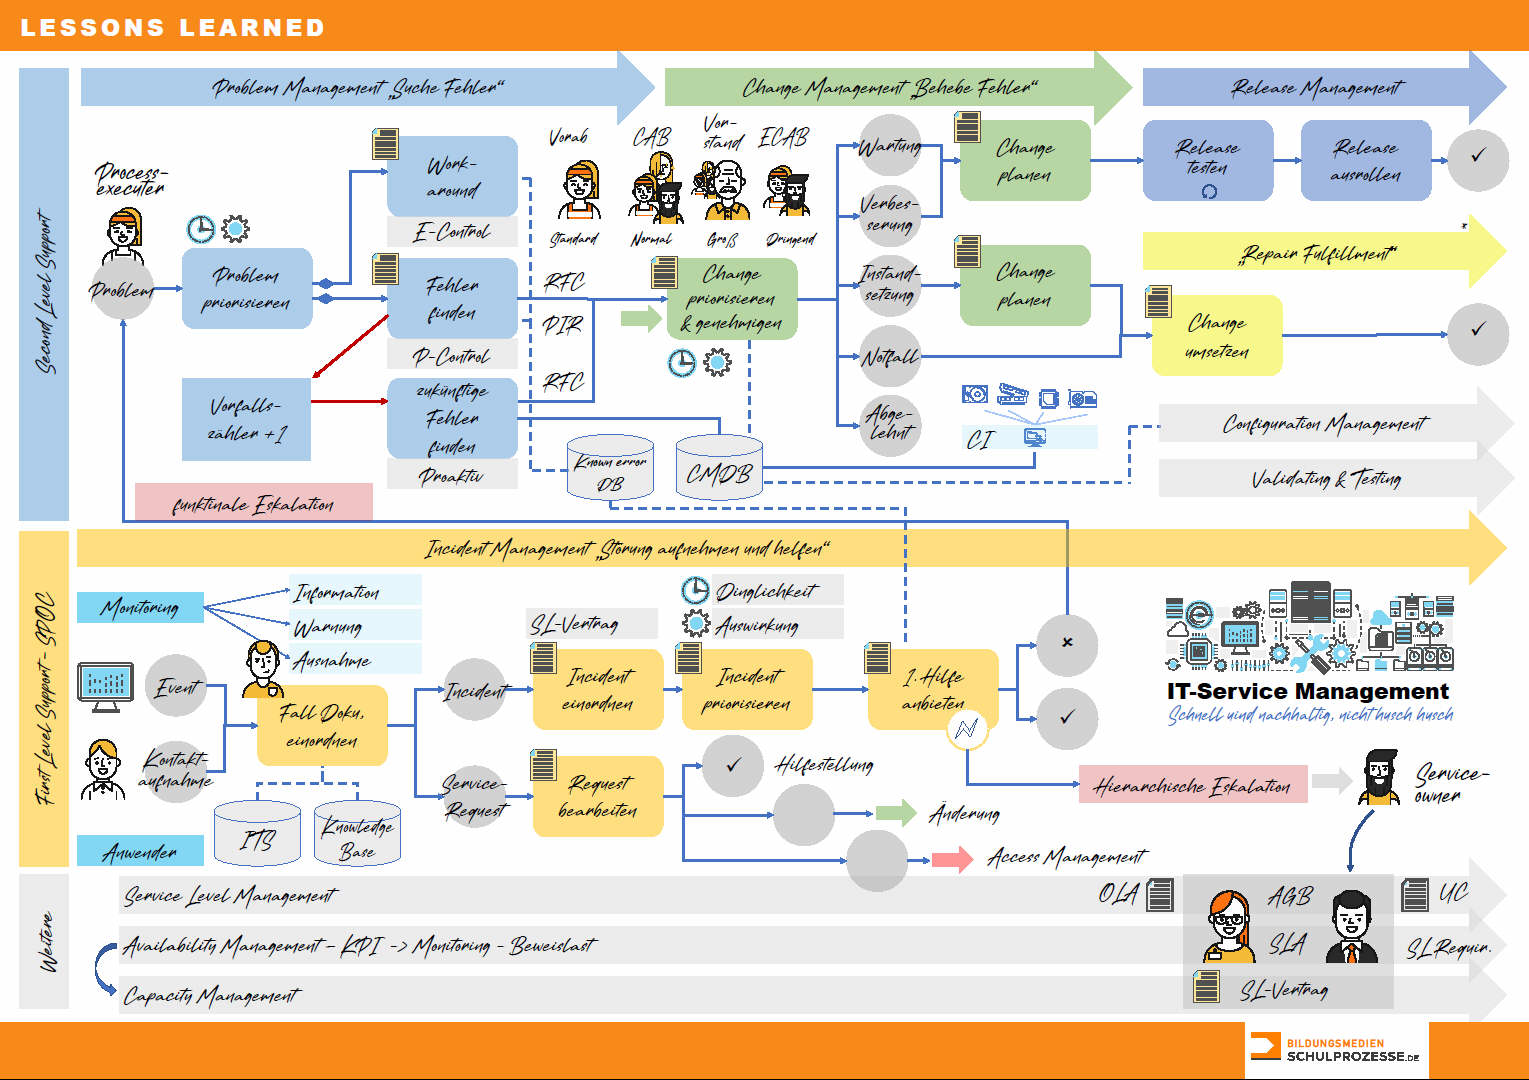
\includegraphics[width=16cm]{serviceanfragen_bearbeiten.jpg}
\end{center}

% SWD
\chapter{Softwaretechnologie und Datenmanagement}
\begin{multicols}{2}

\section{Grundlagen zur Informationssicherheit erarbeiten} % Vom KMS

Im Jahr 2020 wurden in Deutschland 108.474 Fälle von Cyberkriminalität im 
engeren Sinne registriert. Dies entspricht einem Anstieg von ca. 8\% gegenüber 
dem Vorjahr. Zur Cyberkriminalität zählen folgende Delikte: Computerbetrug als 
Cybercrime im engeren Sinne, missbräuchliche Nutzung von 
Telekommunikationsdiensten, sonstiger Computerbetrug, Ausspähen und Abfangen von 
Daten einschließlich Vorbereitungsmaßahmen und Daten-Hehlerei, Fälschung 
beweiserheblicher Daten bzw. Täuschung im Rechtsverkehr sowie 
Datenveränderung/Computersabotage. Fast neun von zehn Unternehmen verschiedener 
Größenordnungen  waren in den Jahren 2020 oder 2021 von Datenklau, Spionage oder 
Sabotage betroffen. Die Schadenssumme betrug 2020 ca. 220 Milliarden Euro. Durch
die COVID-19 Pandemie und eine starke Verbreitung des Home-Office boten sich den 
Kriminellen neue Angriffsflächen. Nach Einschätzung von Firmen stammen etwa 40\%
der Angriffe von Hobby-Hackern. 

\subsection{Aspekte der Speicherung und Verwaltung von Daten}

\section{Technisch-organisatorische Maßnahmen (TOM) und Beiträge zum 
Sicherheitskonzept erstellen} % KMS
\dots

\section{Schutzbedarfsfeststellungen anhand eines Beispielunternehmens des BSI 
vorbereiten} % KMS
\dots

\section{Die Binär- Dezimal- und Hexadezimalsysteme}
\dots

\section{Programmablaufpläne, Struktogramme und Pseudocode}
\dots

\section{Objektorientierte Programmierung}
\dots
\end{multicols}
\end{document}


